\documentclass{article}

\usepackage[utf8]{inputenc}
\usepackage[T1]{fontenc}
\usepackage[english]{babel}   %Engelsk først så norsk, så norsk blir prioritert
\usepackage{graphicx}
\usepackage{amsmath}        %For å kunne skrive matte
\usepackage{listings}       %For å kunne skrive inn kode med fin formatering
\usepackage{multicol}       %Importerer pakken for multikolonner til teksten
\usepackage[margin=2.54cm]{geometry}    %Definerer hva bredden til teksten er
\usepackage{wrapfig}    %Importerer pakken for å ha bildene i teksten
\usepackage[font = small]{caption}
\usepackage{textcomp}
\usepackage{mathrsfs}   %For å få fancy E til bildene

\usepackage{amssymb} %Fra Erlend for å bruke hakemerke?? Vet egt. ikke

%Definerer hyperlinker og dens farger
\usepackage{hyperref}
\hypersetup{
    colorlinks,
    citecolor=blue,
    filecolor=black,
    linkcolor=blue,
    urlcolor=blue
}

%-----------------------------------
\iffalse
%Definerer farger til kodeeksemplene i PDF-en
\usepackage{color}

\definecolor{codegreen}{rgb}{0,0.6,0}
\definecolor{codegray}{rgb}{0.5,0.5,0.5}
\definecolor{codepurple}{rgb}{0.58,0,0.82}
\definecolor{backcolour}{rgb}{0.95,0.95,0.92}

\lstdefinestyle{mystyle}{
    backgroundcolor=\color{backcolour},
    commentstyle=\color{codegreen},
    keywordstyle=\color{magenta},
    numberstyle=\tiny\color{codegray},
    stringstyle=\color{codepurple},
    basicstyle=\footnotesize,
    breakatwhitespace=false,
    breaklines=true,
    captionpos=b,
    keepspaces=true,
    numbers=left,
    numbersep=5pt,
    showspaces=false,
    showstringspaces=false,
    showtabs=false,
    tabsize=2
}

\lstset{style=mystyle}
\fi


%--------------------------------------

\setlength{\parindent}{0pt} %Ingen indent automatisk for nye linjer
%\setlength{\columnsep}{2mm} %Column separation - til multicolumn

%\setlength{\arrayrulewidth}{1mm}   %Hvilken tykkelse tabellene skal ha
\setlength{\tabcolsep}{2mm}     %Lengden mellom hver kolonne
\renewcommand{\arraystretch}{1.5}   %Hvor stor avstand det skal være mellom radene

\iffalse    %midlertidig endre bredden på teksten
If you want to change this temporarily, you can write:
\savegeometry{mydefaultgeometry}
\newgeometry{margin=3in}
And then later you can call:
\loadgeometry{mydefaultgeometry}
\fi

%for å fjerne overskriften "refrences" som kommer automatisk når man bruker bibtex
\usepackage{etoolbox}
\patchcmd{\thebibliography}{\section*{\refname}}{}{}{}

%lage exercises på norsk, slik at det står oppgave. også definere dette som en ny kommando
\newcounter{excount}
\newenvironment{exercise}[1][]{\addtocounter{excount}{1} \noindent {\bf Oppgave
\arabic{excount} \ \ #1}\hspace{2mm}}{\vspace{4mm}}


%----------------------

\usepackage{float}
%\restylefloat{table}

%----------------------

\usepackage{tikz}
\usetikzlibrary{patterns}

\usetikzlibrary{shapes.misc}
% From http://tex.stackexchange.com/questions/123760/draw-crosses-in-tikz
\tikzset{cross/.style={cross out, draw=black, fill=none, minimum size=2*(#1-\pgflinewidth), inner sep=0pt, outer sep=0pt}, cross/.default={3pt}}

\usetikzlibrary{decorations.markings}

%------------------

%dette brukes med \begin{python}
\usepackage{pythonhighlight}

\lstdefinestyle{mystyle}{
    numbers=left,
    numbersep=5pt,
}

\lstset{style=mystyle}


%-----------------------

%figurtekst under, tabelltekst over

%LEGGE TIL STJERNER VED SECTION FJERNER NUMMERERINGEN!!!!!!!!!!!!!!!!!!!!!!!!!!!!!!!!
%men da syntes ikke avsnittene i innholdsfortegnelsen!!!!!!!!!!!!!!!!!!!!!!!!!!!!!!!!

%------------------------------------------------------------------------------

\begin{document}

\addtocounter{page}{0}

\title{Project A20 \\
      \large FYS-MENA4111}
\date{\today \\
    \vspace{1mm}
    \large Week 44-48}

\author{Erlend Tiberg North \& Alexandra Jahr Kolstad}

\maketitle


%\newpage

%--------------- Her starter skrivingen ---------------------------------------

%\begin{multicols}{2}


%---------------------- Abstract -----------------------------------------
\vspace{1cm}


\begin{center}

{\Large\textbf{Abstract}} \label{sec:Abstract} \\

    Quinizarin can function as an organic sensetizer in an upconversion system. In ALD the organic molecule can possibly be deposited in a matrix of lanthanide flouride, to increase the efficiency of the upconversion process in the material. To see how this efficiency can increase and what energy levels can be absorbed by the material, it is wise to investigate the electronic band structure of the molecule. This paper will look in to Quinizarin's own electronic properties, as well as, Quinizarin with lanthanides replacing one a Hydrogen atom, to emulate Quinizarin inside the structure in a simple way.

    \vspace{1cm}

\end{center}


\newpage

%-------------------- Table of contents -----------------------------------
\vspace{1cm}

\tableofcontents

\vspace{1cm}

%---------------------------------------------------------------------------------

\textbf{Ting å gjøre:}
\begin{itemize}
    \item lage en mappe på saga for begge
    \subitem \textbf{done}
    \item skaffe POSCAR, jobfile og INCAR (de andre følger fra disse)
    \subitem \textbf{done}
    \item sjekke at den konvergerer (decent ENCUT og KPOINTS)
    \subitem \textbf{done}
    \subitem The data shows that we should use 450eV for ENCUT as that is the 1st job with a difference less than 3meV.
    \subitem For k-density we see that even the lowest value, 1.0, is within 3 meV (1.0 gives around 1.75 meV), so this can be used. However, the data shows that 3.0 is below 1 meV, with 4.0 being identical in energy to 5.0. This can possibly be discussed in group, but 1.0 should technically be enough for k-density.
    \item relaxe POSCAR og static etter relax POSCAR
    \subitem \textbf{done}
    \item total og relativ energi (fra static etter relax)
    \subitem \textbf{done}
    \item DOS og LDOS
    \subitem \textbf{done}
    \item romlig elektronstruktur; 3D-plot av ladningstetthet (VESTA)
    \subitem \textbf{done}
    \item bytte ut hydrogen i alkoholgruppen med lantanoidatomer (Yb, Nd, Tm og Y)
    \subitem \textbf{done}
    \item relaxe POSCAR og static etter relax POSCAR
    \subitem \textbf{done}
    \item total og relativ energi (fra static etter relax)
    \subitem \textbf{done}
    \item DOS og LDOS
    \subitem \textbf{done}
    \item romlig elektronstruktur; 3D-plot av ladningstetthet (VESTA)
    \subitem \textbf{done}
\end{itemize}

\vspace{1cm}

\textbf{Ting å ha i \LaTeX:}
\begin{itemize}
    \item abstrakt
    \subitem \textbf{done}
    \item kort introduksjon av materialet
    \subitem \textbf{done}
    \item kort om metode, valg av paramtere (CUTOFF, etc)
    \subitem \textbf{done}
    \item presentasjon av de viktigste resultatene
    \subitem \textbf{WIP}
    \item diskusjon av hvordan resultatene kan tolkes, f.eks. sammenligne til eksperimenter eller tidligere beregninger i litteraturen
    \subitem \textbf{WIP}
    \item konklusjon/oppsummering
    \item kilder
    \item appendix ?
\end{itemize}

\vspace{1cm}

\textbf{\large{OBS: husk å lagre bilder for rapporten og presentasjonen mens man gjør beregningene}}

\section{Introduction}  \label{sec:Introduction}

    Photons can be used for many things. However, not all photons are created equal. They come in many different energies, and not all energies are as simple to absorb. A way to increase the efficiency of photon-absorbing materials is by modifying it so that it can absorb photons with a low energy, collect that energy, and re-emit the photon with higher energy. This is known as up-conversion and has many uses. One use is to increase the efficiency of solar panels by allowing it to collect more of the sunlight, where the up-conversion system can be a thin-film on the top of the panel. A different use is to increase the energy to the point where the emitted photon can become ionizing and work as a bacteria or virus killer.\\

    Up-conversion is a phenomenon where incoming photons are re-emitted with a higher energy than they entered with. The photons excite electrons in a material, and by conduction of those electrons they can move to other atoms, where they are further excited. The electron ends up in a high energy state and de-excites releasing all the energy. However, the process can be very inefficient due to narrow energy bands in the material. A form of increasing this efficiency is by adding a material with a wide energy band to allow absorption of photons with more varied energy.\\

    This paper will focus on an organic compound known as Quinizarin. The compound is an organic dye and has a broad energy band. This means it can absorb a broad spectrum of photons energies. The excited electrons from this energy band can move to the actual up-conversion system and hereby increase the efficiency of the up-conversion. The planned up-conversion system will consist of Quinizarin as an organic sensitizer, Nd+3 and Yb+3 as electron migrators (transporting the electrons to the site of de-excitation), and Tm+3 as accumulator and activator (collecting excited electrons and up-converting them, and de-excitation site for said electrons). The system is planned to be inserted into a matrix of YbF3 or possibly YF3.\\

    Since Quinizarin is such an important piece of the system it is wise to know how it interacts with the other materials. This study will therefore investigate how Quinizarin's electronic band structure changes when the Hydrogen in the alcohol group is replaced with different atoms. In this case: Yb, Nd, Tm and Y. See %figure~(\ref{fig:Quinizarin-X} for an illustration).\\

\iffalse
    \begin{figure}[H]
        \centering
        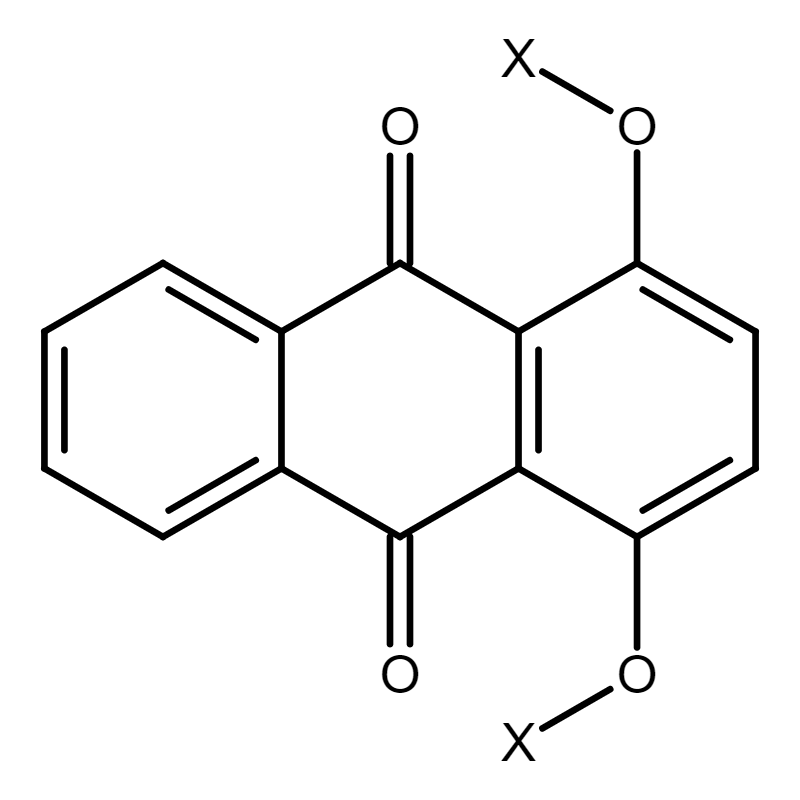
\includegraphics[width = 11cm]{../fig/quinizarin-x.png}
        \caption{Molecular structure of Quinizarin with H in -OH replaced with atom X. X can be H, Y, Yb, Nd or Tm. Structure drawn with online illustrator from \href{https://chem-space.com/search}{Chem-Space}.}
        \label{fig:Quinizarin-X}
    \end{figure}
\fi

\vspace{1cm}

\section{Method}    \label{sec:Method}

  The supercomputer Saga contains many different POSCAR-files for a wide range of structures. Unfortunately for us, Quinizarin was not included. Therefore we had to make our own POSCAR-file. This was done by drawing the structure in an organic compound structure program we found on the internet: \href{https://molview.org}{MolView}. This site lets the user draw organic structures with many varying features, and it also lets the user export the data as a \texttt{.mol}-file. A \texttt{.mol}-file has a similar structure with a POSCAR-file, which let us easily make the POSCAR-file for Quinizarin. \\

  The coordinates of the atoms in the \texttt{.mol}-file were put in a POSCAR file with Direct coordinates. We added a unit cell and, and opened it in VESTA. In order to make the plane-waves more stable for the calculations, we inserted a vacuum distance in each direction of 12 Å. \\

  To differentiate the two Hydrogen-atoms in the alcohol-groups from the other Hydrogen-atoms, we had to find their positions somehow. This was done in the program GeoGebra, by plotting each atom with their positions in 3D. We found that the Hydrogen-atoms were number 25 and 26 in POSCAR. In hindsight, we discovered that this would be easier to do in VESTA. \\

  In this project we will compare the basic Quinizarin with Quinizarin with both Yttrium (Y) and Ytterbium (Yb) substituted in the Hydrogen-positions described in the subsection above. Therefore we had to make in total three POSCAR-files for the three structures. This was done by opening POSCAR in Emacs and changing the two last atoms given in the file to the substitution-atoms. After that we ran in to issues with relaxing the structure, and so went to the ICSD database to find a decent distance between the new atoms and oxygen. We used approximately 2.3 Å in distance, and that worked well for relaxing the structure. \\


  \subsection{Convergence}  \label{sec:Convergence}

    Testing for convergence of energy and k-point is important to determine if the variables in INCAR or KPOINTS are good enough to be used for further calculations, mostly to ensure decent and applicable results. If the error is less than $1\cdot 10^{-3}$ the calculation can be considered converged. \\

    The testing of convergence is done by performing VASP calculations with different values of either energy-cutoff (ENCUT) or k-point density. For this project the energy convergence testing was done for ENCUT between 300 and 900 eV, with 50 eV steps. The k-point convergence testing was done for k-point density between 1.0 and 6.0, with 1.0 difference. For the aforementioned test the value for ENCUT was decided from the energy convergence test. \\


  \subsection{Relax}

    A relaxing calculation is performed to minimize the max force of the material. This is done by moving the atoms to find the optimal atom positions for the structure. \\

    We performed the relaxation calculation once for each structure. \\


  \subsection{Static}

    A static calculation is a calculation in which atoms are held at their original positions. These are often used for obtaining a converged energy, as calculations that relax the structure are less safe to use for this.\\

    In this project we have performed static calculations both before and after performing ionic relaxation. The static calculations that were performed before relaxation were to see how the energies changed between before and after relaxation. \\


  \subsection{DOS}

    A plot of density of states shows the at what levels the energy bands, or orbitals, exists and how broad they are. A band with a high density of states allows for more electrons to occupy it, whereas a band with a low density of states allows for fewer. The density of states is generally plotted against the energy, and peaks in the plot show how many electrons are allowed to exist at a specific energy. An energy gap is shown by two peaks separated by a void. The size of the void (span in energy) is the height of the energy gap. \\

    For obtaining a plot of density of states we ran the script dosplot.py for the values generated by the post-relaxation static calculations. This ensured that the values were converged and safe to use. dosplot.py reads the DOSCAR-file and plots the values in an easy-to-read format. \\


  \subsection{Bang gap}

    The density of states plots show where the band gap is located, but it does not give the numerical value. VASP has the command \texttt{bandgap} specifically for this, hence we used this to find the numerical value of the band gap for the structures. \\


  \subsection{Charge density}

    The charge density of a structure shows how the charge is distributed around the atoms in that structure. A plot of the charge density therefore shows how many electrons the different atoms attract. To plot the charge density the file CHGCAR, after a completed VASP calculation, is copied over to VESTA, and then visualized.


\vspace{1cm}

\section{Results}   \label{sec:Results}

  \subsection{Convergence of energy}

     The energy convergence tests were run as described in Section \ref{sec:Convergence}. After the runs were completed we looked at vaspout from each of the runs. The total energy per atom, or TOTEN/atom, was plotted against the cutoff energy and this is shown in Figure~(\ref{fig:convergence_energy.png}). \\

     Figure~(\ref{fig:convergence_energy_difference.png}) shows the difference in energy from one value to the next. This means, the value of ENCUT=300 is the difference in total energy going a cutoff energy of 300 eV to 350 eV. \\



    \begin{figure}[H]
      \centering
      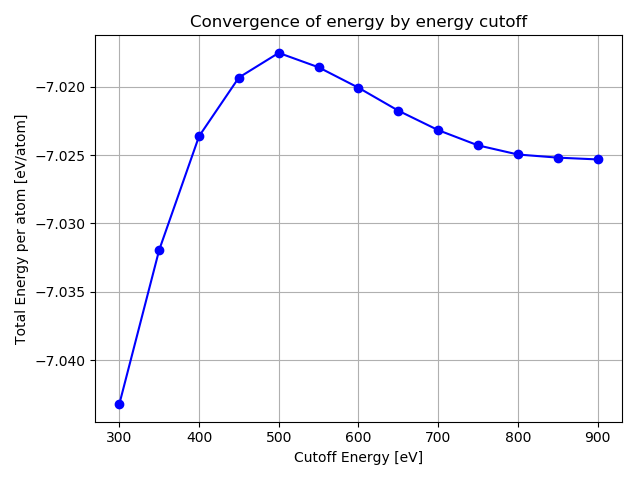
\includegraphics[width = 11cm]{../fig/convergence_energy.png}
      \caption{Plot of energy convergence for Quinizarin, with ENCUT ranging from 300 eV to 900 eV. }
      \label{fig:convergence_energy.png}
    \end{figure}

    \begin{figure}[H]
      \centering
      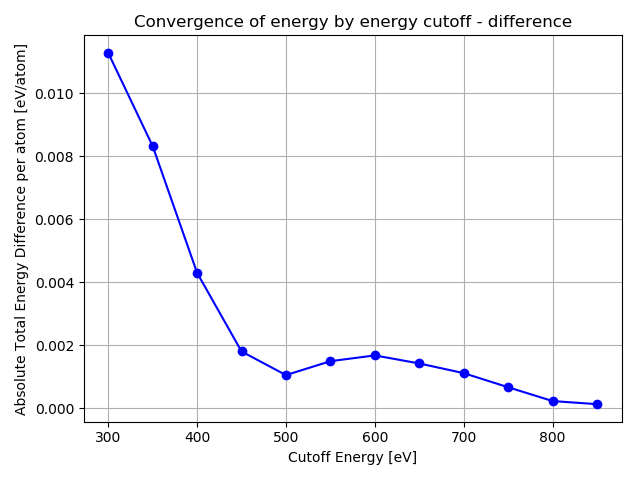
\includegraphics[width = 11cm]{../fig/convergence_energy_difference.png}
      \caption{Plot of the difference in energy convergence for Quinizarin, given by ENCUT. }
      \label{fig:convergence_energy_difference.png}
    \end{figure}


  \subsection{Convergence of k-points}

    For the convergence of k-points the span of values were used as described in Section \ref{sec:Convergence}. Figure~(\ref{fig:convergence_kpoints.png}) shows how the total energy changes as k-density increases. Like with energy, the difference has also been plotted, and this is shown in Figure~(\ref{fig:convergence_kpoints_difference.png}).


    \begin{figure}[H]
        \centering
        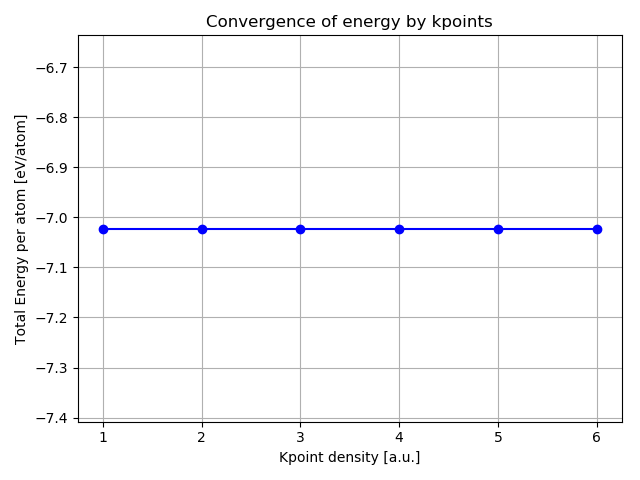
\includegraphics[width = 11cm]{../fig/convergence_kpoints.png}
        \caption{Plot of energy convergence for Quinizarin, with k-point density ranging from 1 to 6. }
        \label{fig:convergence_kpoints.png}
    \end{figure}

    \begin{figure}[H]
        \centering
        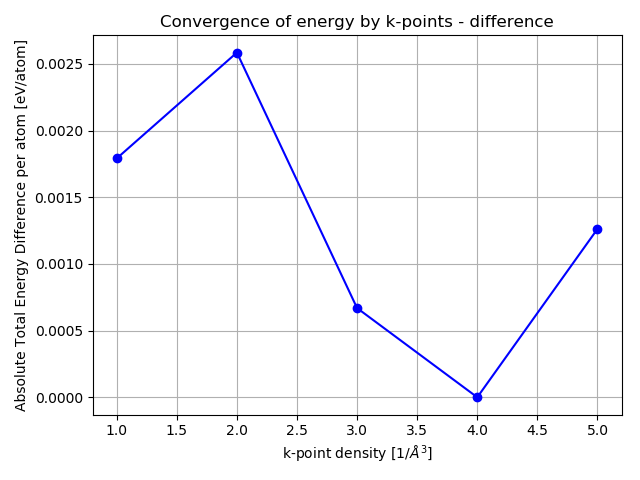
\includegraphics[width = 11cm]{../fig/convergence_kpoints_difference.png}
        \caption{Plot of the difference in energy convergence for Quinizarin, given by k-point density. }
        \label{fig:convergence_kpoints_difference.png}
    \end{figure}


  \subsection{Quinizarin}

    \subsubsection{Relaxing the structure}

      The initial static calculation of Quinizarin gave a CONTCAR as shown in Figure~(\ref{fig:basic_staticbefore_CONTCAR}). \\

      After relaxing the structure and performing a new static calculation, CONTCAR looked as shown in Figure~(\ref{fig:basic_staticafter_CONTCAR}). We do not show CONTCAR from the actual ionic relaxation as it is identical to the post-relaxation static calculation.


      \begin{figure}[H]
        \centering
        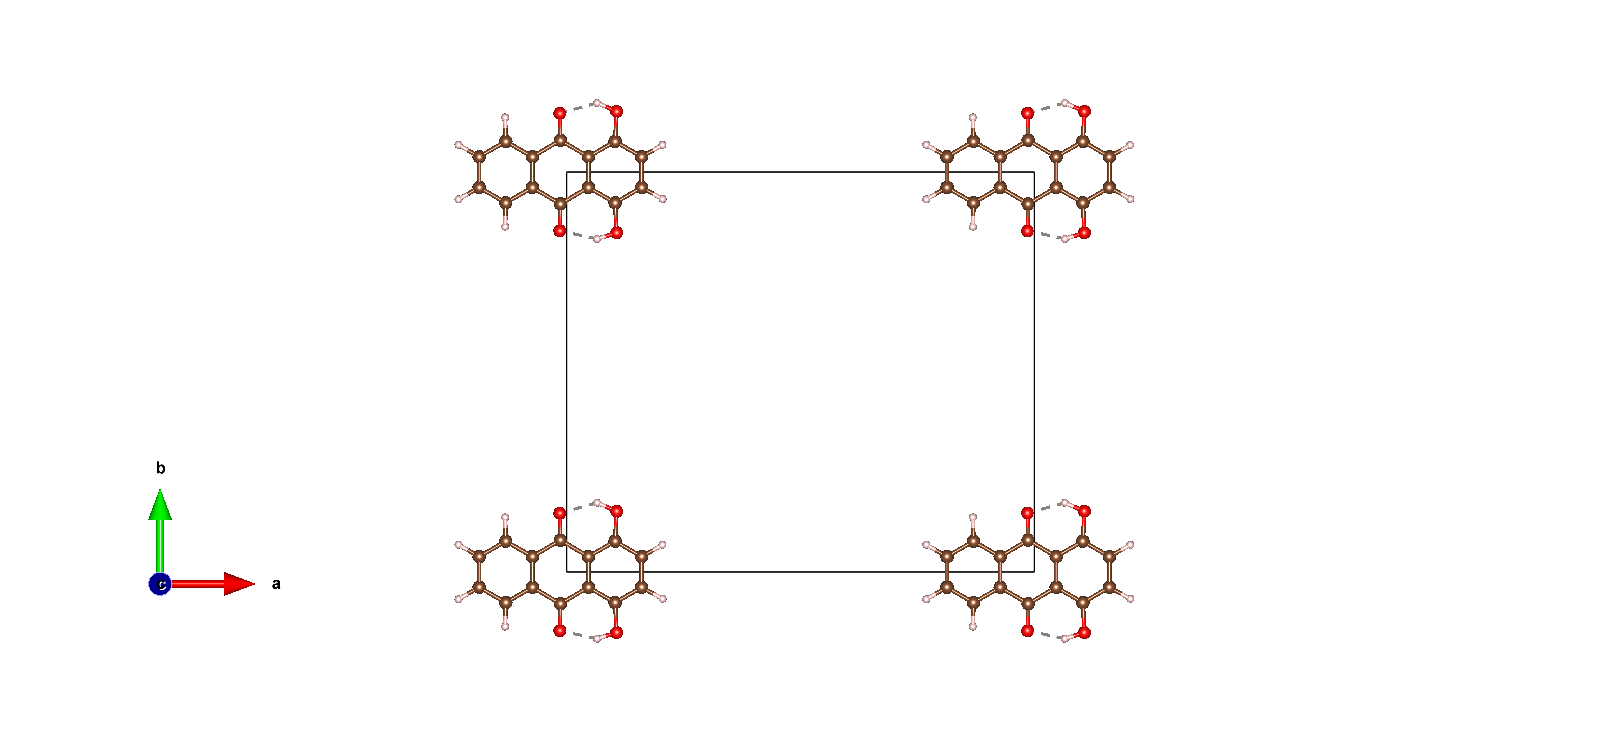
\includegraphics[width = 11cm]{../fig/basic_staticbefore_CONTCAR.png}
        \caption{Structure of Quinizarin for static VASP calculation. }
        \label{fig:basic_staticbefore_CONTCAR}
      \end{figure}

      \begin{figure}[H]
        \centering
        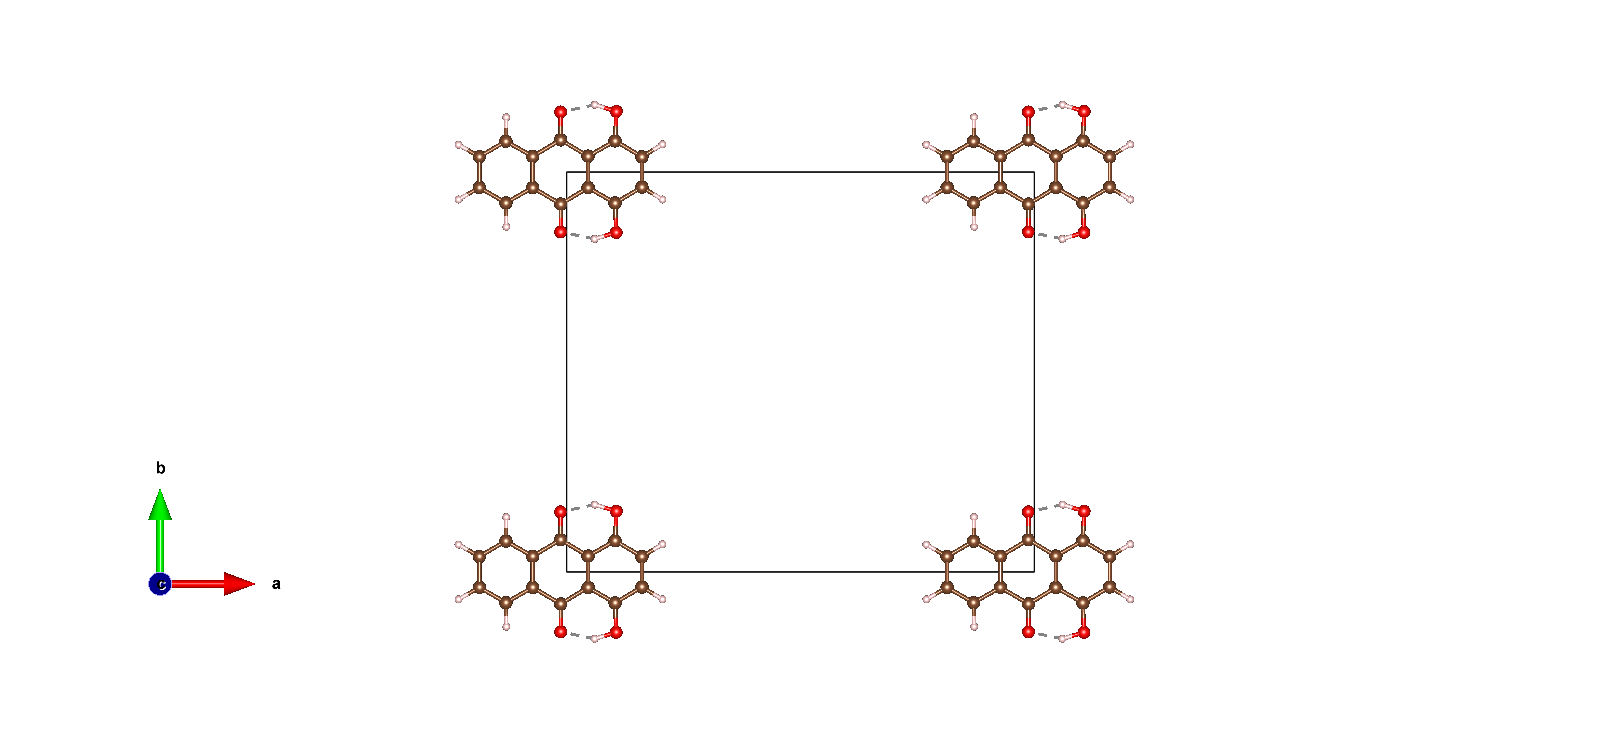
\includegraphics[width = 11cm]{../fig/basic_staticafter_CONTCAR.png}
        \caption{Structure of Quinizarin for static VASP calculation after relaxed calculation. }
        \label{fig:basic_staticafter_CONTCAR}
      \end{figure}


    \subsubsection{Total and relative energies}

      As can be seen in Table~(\ref{tab:TOTENquinizarin}), there was a difference in total energies. This turned out to be 0.015 eV in relative energy difference.

      \begin{table}[H]
        \centering
        \caption{Total energy per atom for Quinizarin}
        \label{tab:TOTENquinizarin}
        \begin{tabular}{|c|c|}
            \hline
            Calculation & Total energy per atom [eV/atom]  \\
            \hline \hline
            staticbefore & $-7.019$ \\
            staticafter & $-7.034$ \\
            \hline
        \end{tabular} \\
        \hspace{0pt}\\
    \end{table}

    \subsubsection{Total and local density of states}

      In Figure~(\ref{fig:basic_TDOS_2} we can see the total density of states of the Quinizarin molecule. Figure~(\ref{fig:basic_LDOS25_2} shows the local density of states for the Hydrogen atom in the lower alcohol group, whereas Figure~(\ref{fig:basic_LDOS26_2} shows the local density of states for the Hydrogen atom in the upper alcohol group.
      It is important to note that these figures are zoomed in around the fermi-level. To see the full pictures, see Figure~(\ref{fig:basic_TDOS_1}), Figure~(\ref{fig:basic_LDOS25_1}) and Figure~(\ref{fig:basic_LDOS26_1}) in \ref{sec:Appendix}. \\


      \begin{figure}[H]
        \centering
        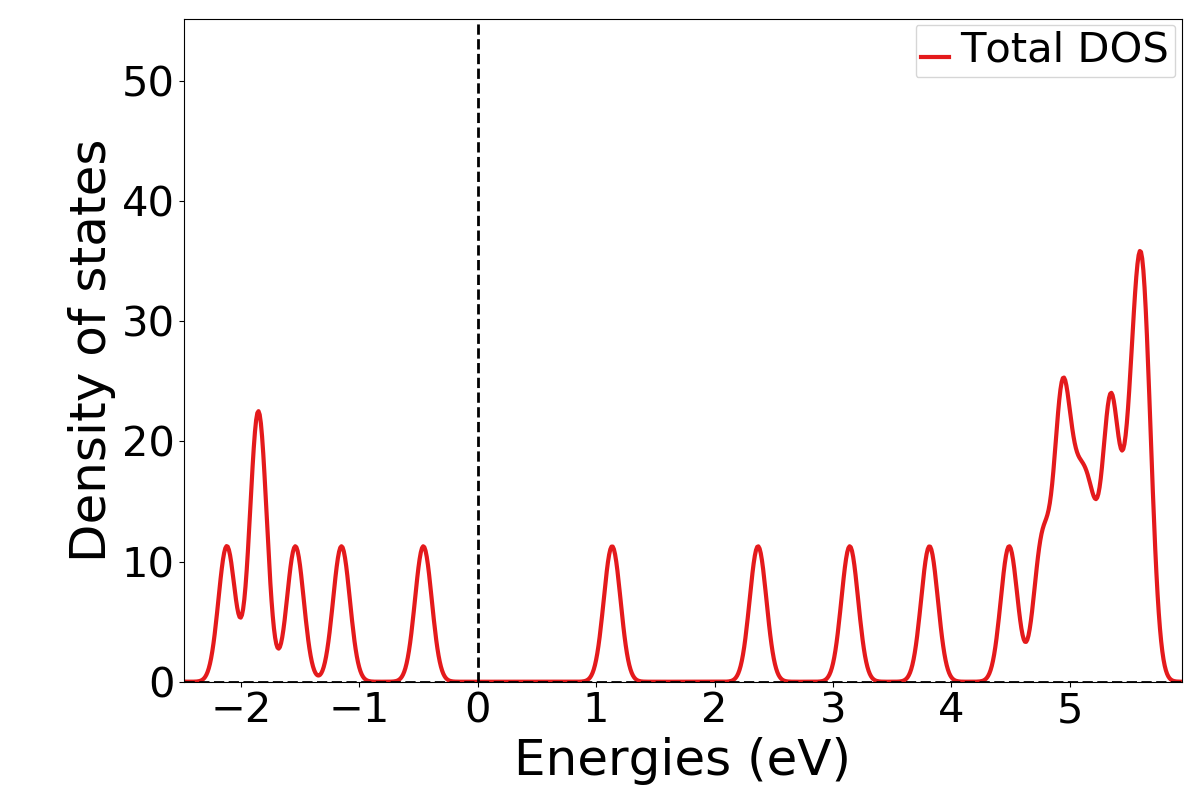
\includegraphics[width = 11cm]{../fig/basic_TDOS_2.png}
        \caption{Plot of total DOS for Quinizarin, zoomed in for energies between 4.0 eV and 8.0 eV. }
        \label{fig:basic_TDOS_2}
      \end{figure}

      \begin{figure}[H]
        \centering
        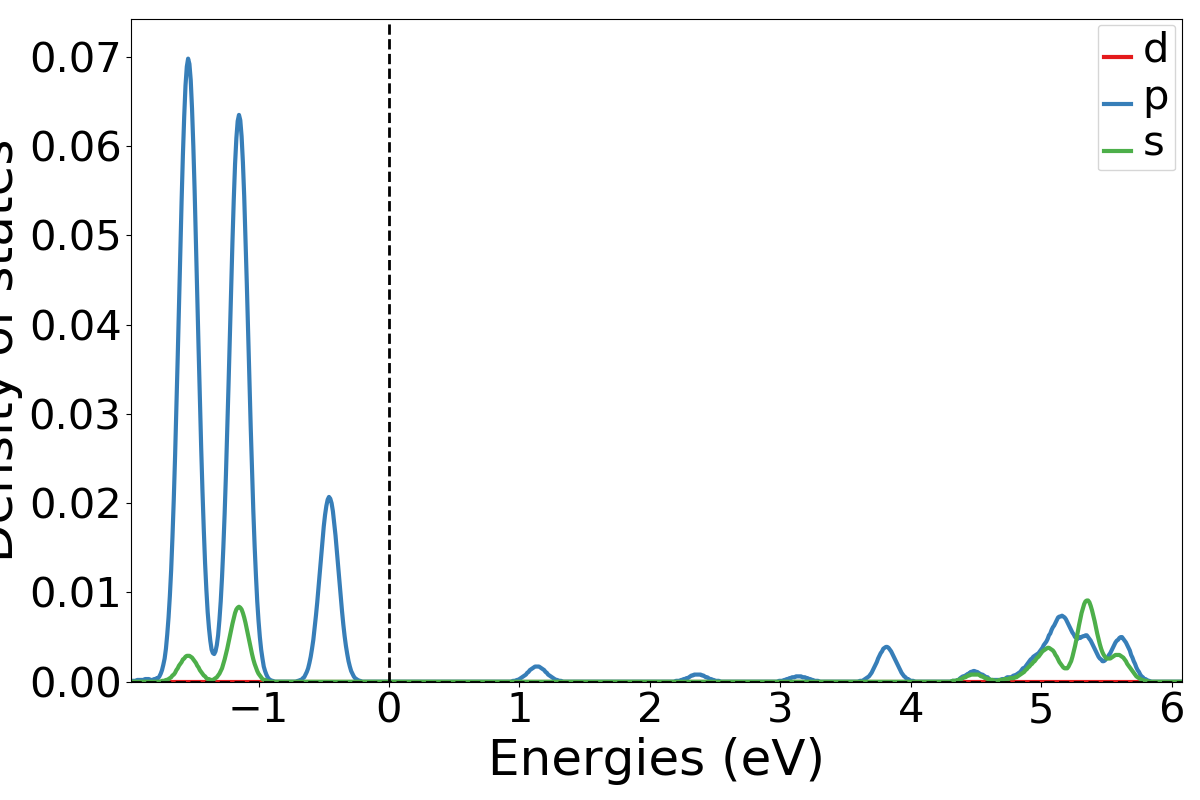
\includegraphics[width = 11cm]{../fig/basic_LDOS25_2.png}
        \caption{Plot of local DOS for atom number 25(H in alcohol-group) for Quinizarin, zoomed in for energies between 4.0 eV and 8.0 eV. }
        \label{fig:basic_LDOS25_2}
      \end{figure}

      \begin{figure}[H]
        \centering
        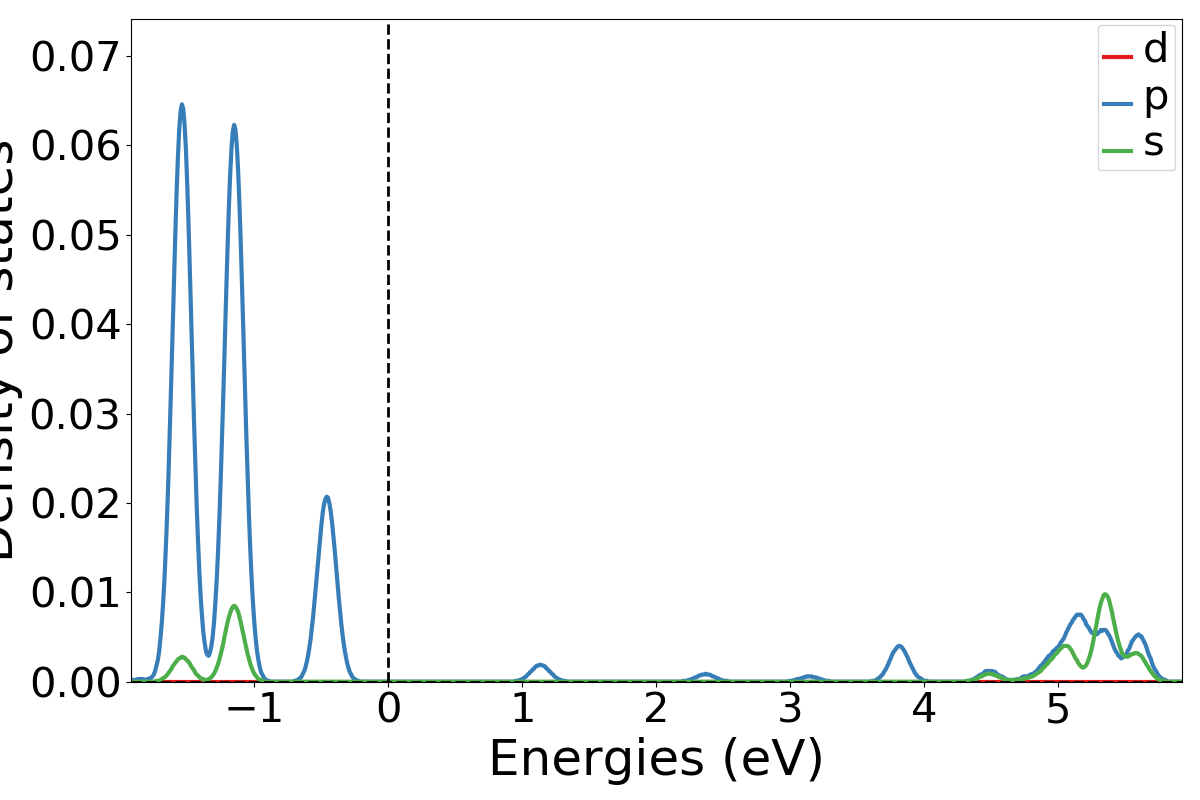
\includegraphics[width = 11cm]{../fig/basic_LDOS26_2.png}
        \caption{Plot of local DOS for atom number 26(H in alcohol-group) for Quinizarin, zoomed in for energies between 4.0 eV and 8.0 eV. }
        \label{fig:basic_LDOS26_2}
      \end{figure}

    \subsubsection{Band gap}

      \begin{table}[H]
        \centering
        \caption{Band gap, valance band maximum and conduction band minimum for Quinizarin with static calculations. }
        \vspace{0mm}
        \label{tab:bandgapquinizarin}
        \begin{tabular}{|c|c|c|c|}
            \hline
            Calculation & Band gap [eV] & VBM [eV] & CBM [eV]  \\
            \hline \hline
            Before relax & $1.773$ & $-5.335$ & $-3.562$ \\
            After relax & $1.594$ & $-5.313$ & $-3.720$ \\
            \hline
        \end{tabular} \\
        \hspace{0pt}\\
      \end{table}


    \subsubsection{Charge density}

      The charge density for the static calculation after relaxation can be shown in Figure~(\ref{fig:basic_staticafter_CHGCAR}. The charge density before relaxation is shown in Figure~(\ref{fig:basic_staticbefore_CHGCAR}).

      \begin{figure}[H]
        \centering
        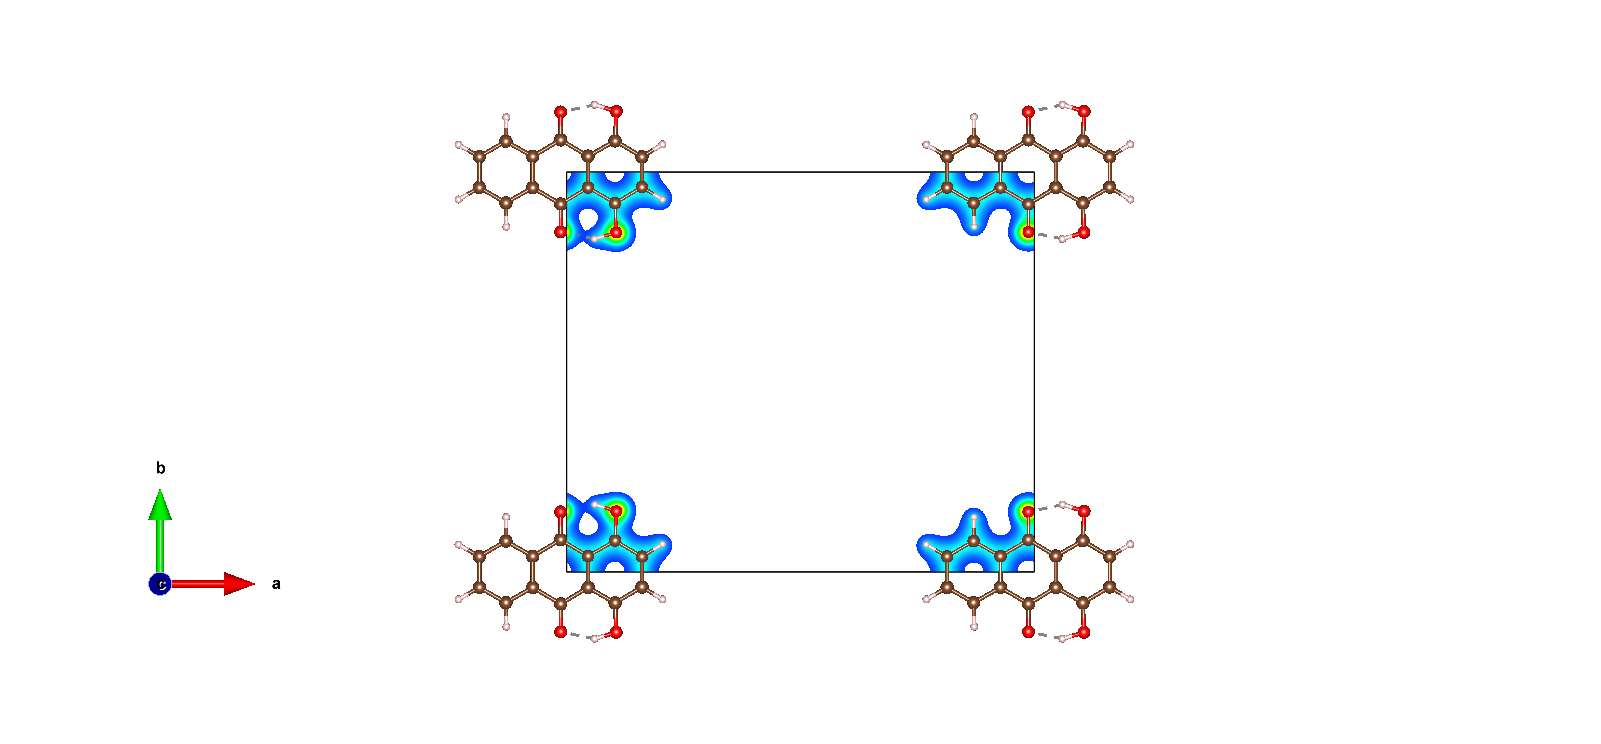
\includegraphics[width = 11cm]{../fig/basic_staticafter_CHGCAR.png}
        \caption{Charge density of Quinizarin for static VASP calculation after relaxed calculation. }
        \label{fig:basic_staticafter_CHGCAR}
      \end{figure}

      \begin{figure}[H]
        \centering
        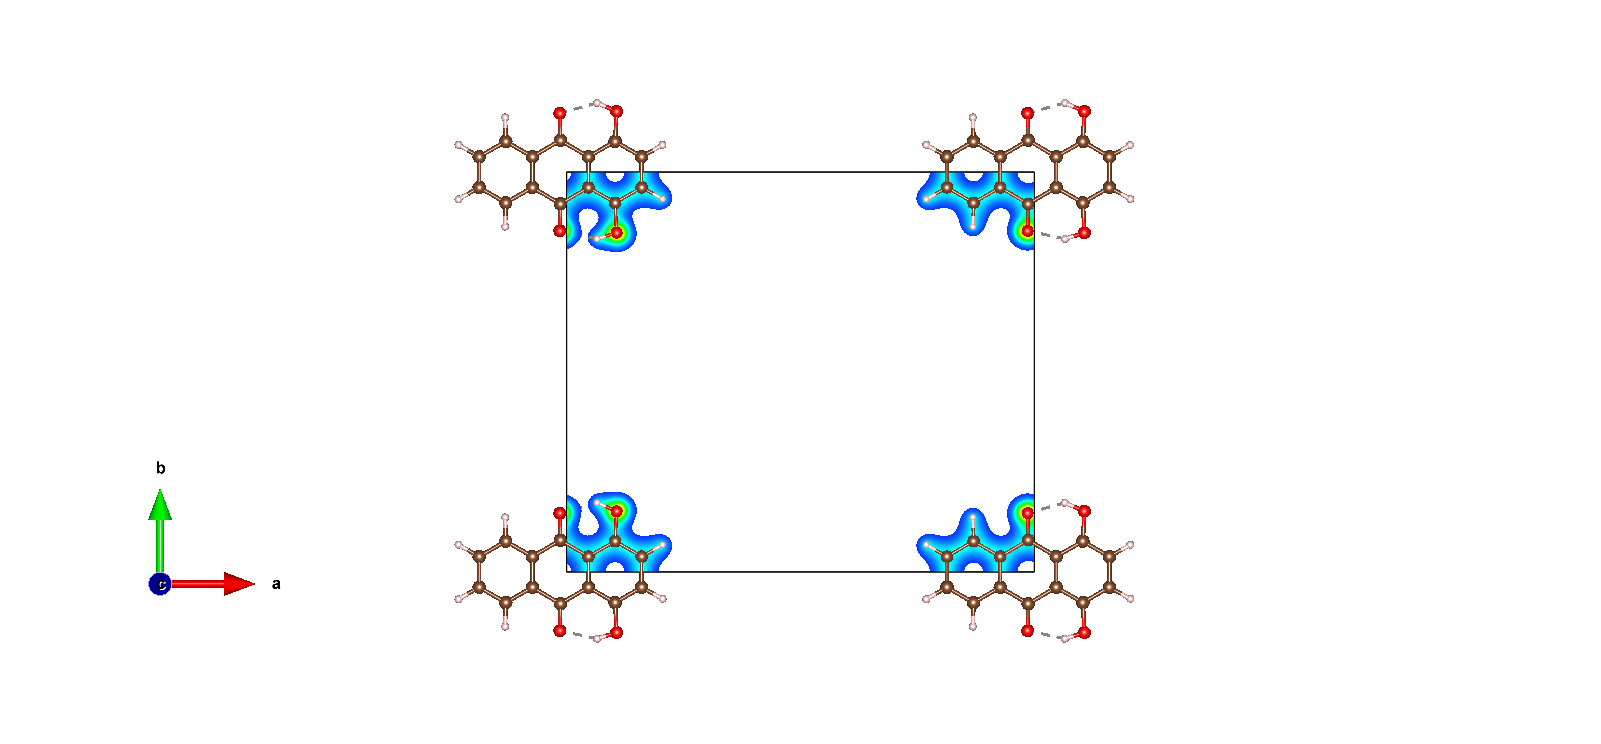
\includegraphics[width = 11cm]{../fig/basic_staticbefore_CHGCAR.png}
        \caption{Charge density of Quinizarin for static VASP calculation. }
        \label{fig:basic_staticbefore_CHGCAR}
      \end{figure}


  \subsection{Quinizarin with Yttrium}

    \subsubsection{Relaxing the structure}


      \begin{figure}[H]
        \centering
        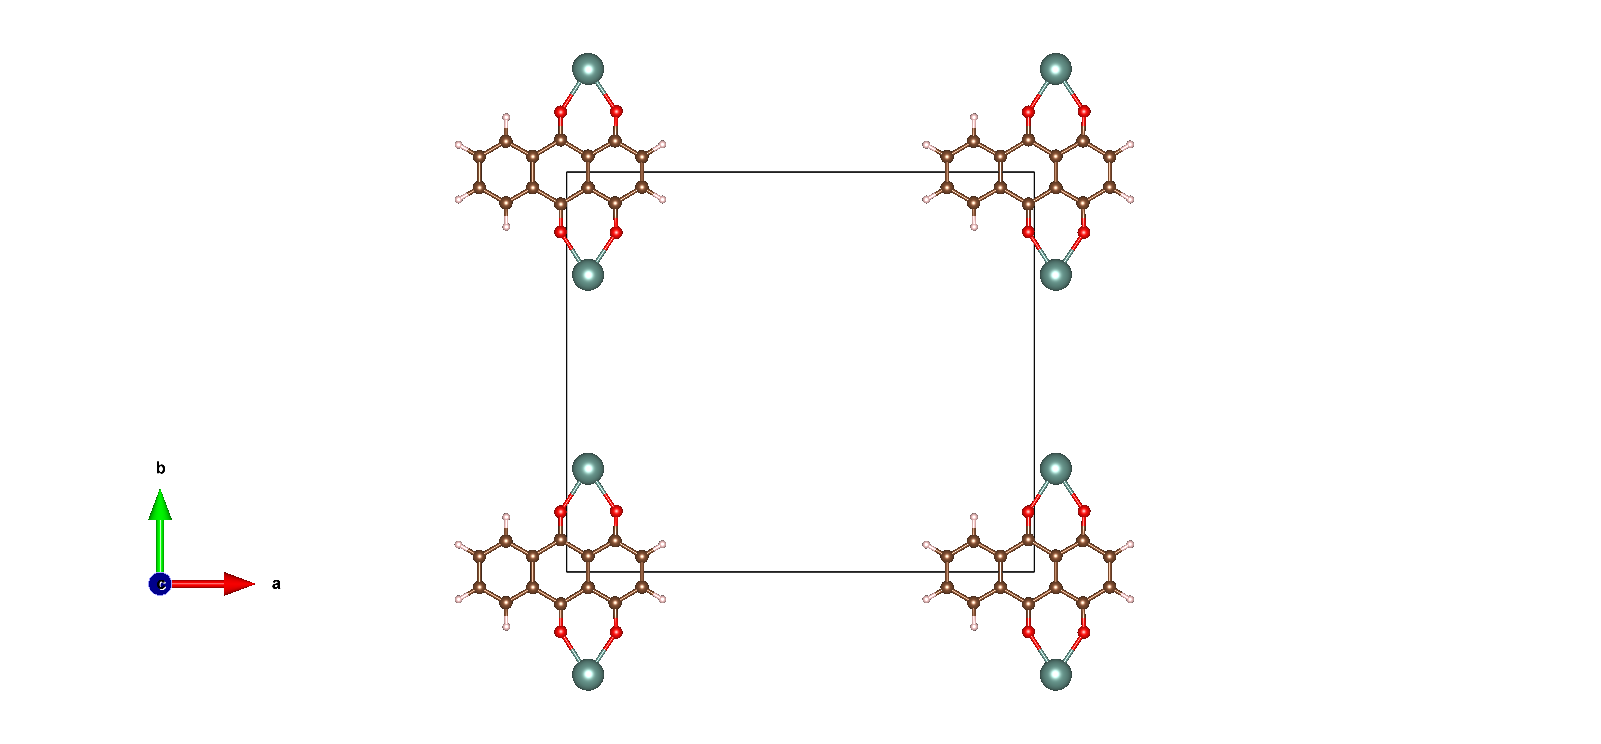
\includegraphics[width = 11cm]{../fig/Y_staticbefore_CONTCAR.png}
        \caption{Structure of Quinizarin with Yttrium for static VASP calculation. }
        \label{fig:Y_staticbefore_CONTCAR}
      \end{figure}

      \begin{figure}[H]
        \centering
        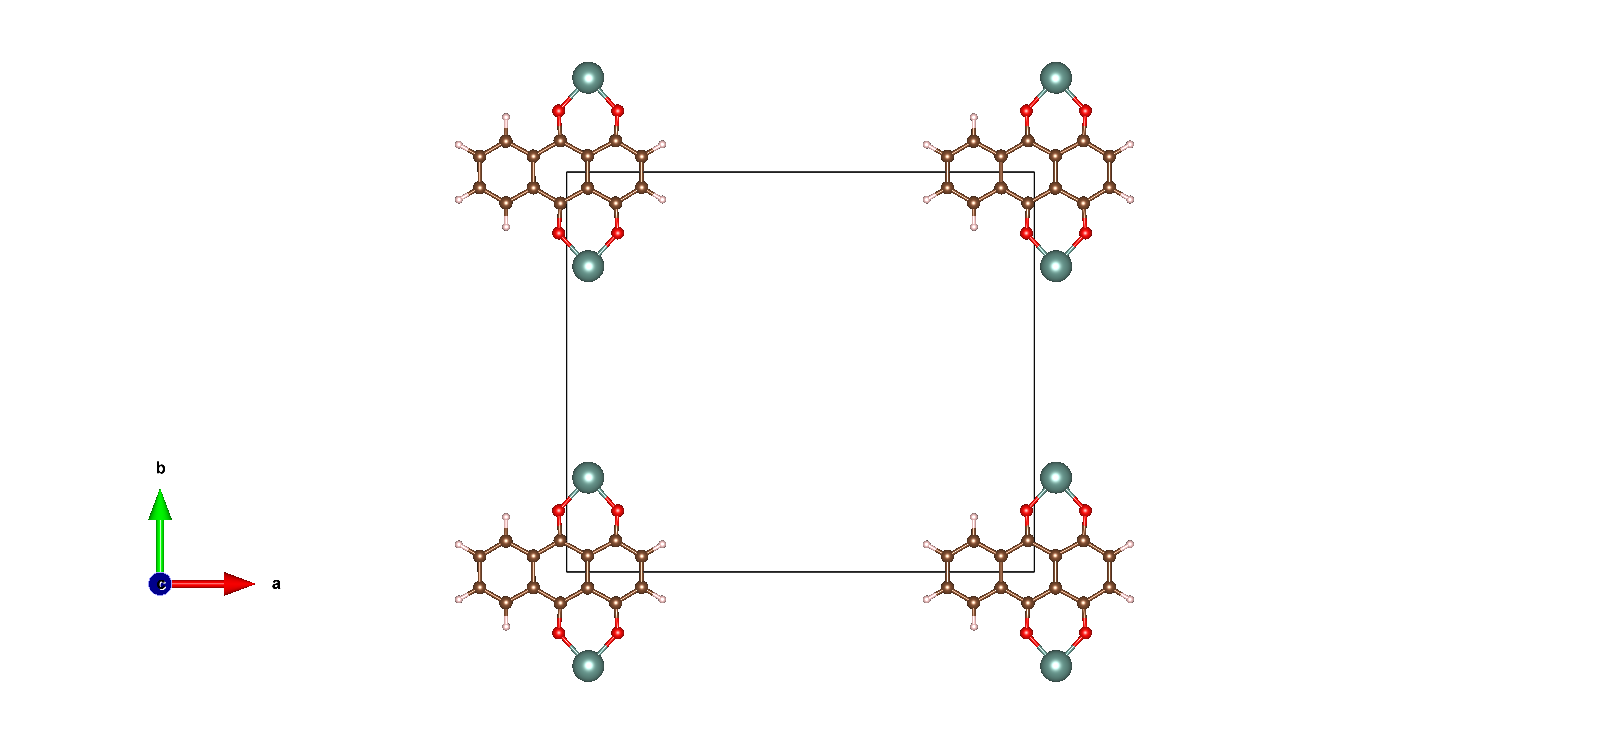
\includegraphics[width = 11cm]{../fig/Y_staticafter_CONTCAR.png}
        \caption{Structure of Quinizarin with Yttrium for static VASP   calculation after relaxed calculation. }
        \label{fig:Y_staticafter_CONTCAR}
      \end{figure}


    \subsubsection{Total and relative energies}

      Table of TOTEN for each and TOTEN relative to each other

      \begin{table}[H]
        \centering
        \caption{Total energy per atom for Quinizarin with Yttrium. }
        \vspace{0mm}
        \label{tab:TOTENY}
        \begin{tabular}{|c|c|}
            \hline
            Calculation & Total energy per atom [eV/atom]  \\
            \hline \hline
            staticbefore & $-7.167$ \\
            staticafter & $-7.276$ \\
            \hline
        \end{tabular} \\
        \hspace{0pt}\\
      \end{table}


    \subsubsection{Total and local density of states}

      TDOS and LDOS graphs

      \begin{figure}[H]
        \centering
        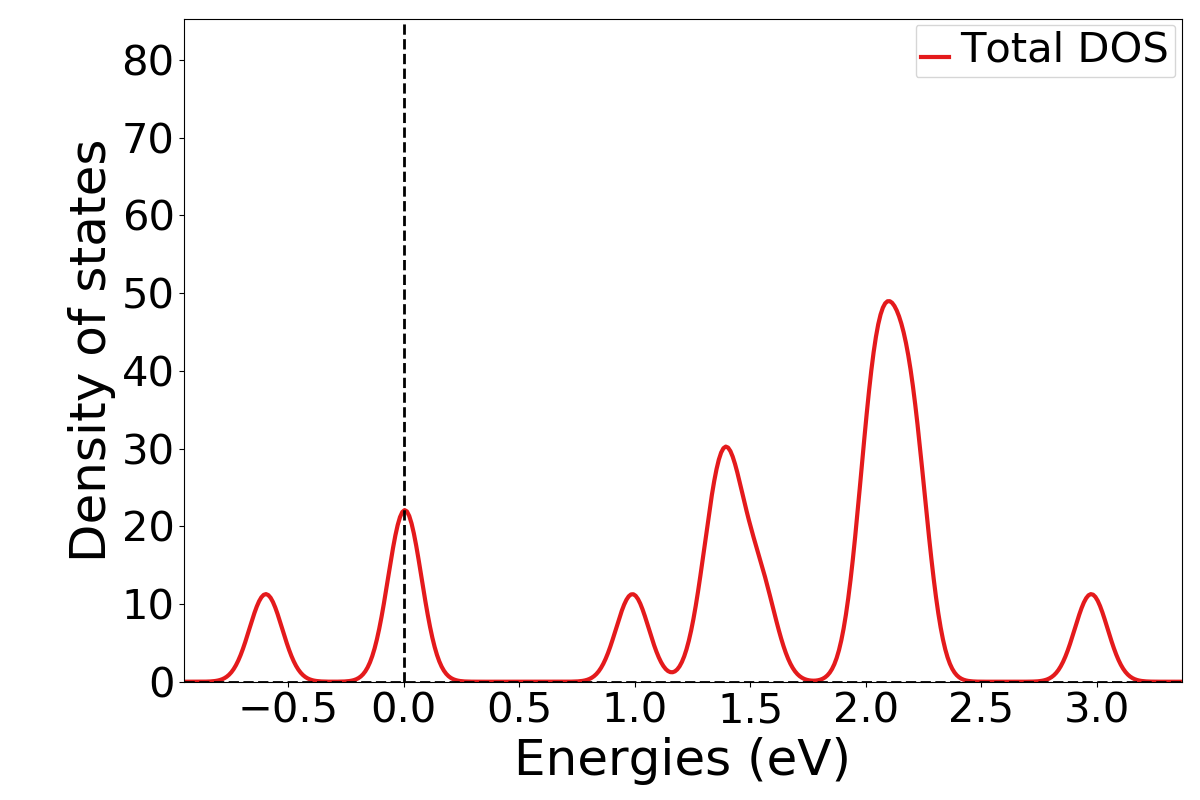
\includegraphics[width = 11cm]{../fig/Y_TDOS_2.png}
        \caption{Plot of total DOS for Yttrium, zoomed in for energies between 0.0 eV and 4.5 eV. }
        \label{fig:Y_TDOS_2.png}
      \end{figure}

      \begin{figure}[H]
        \centering
        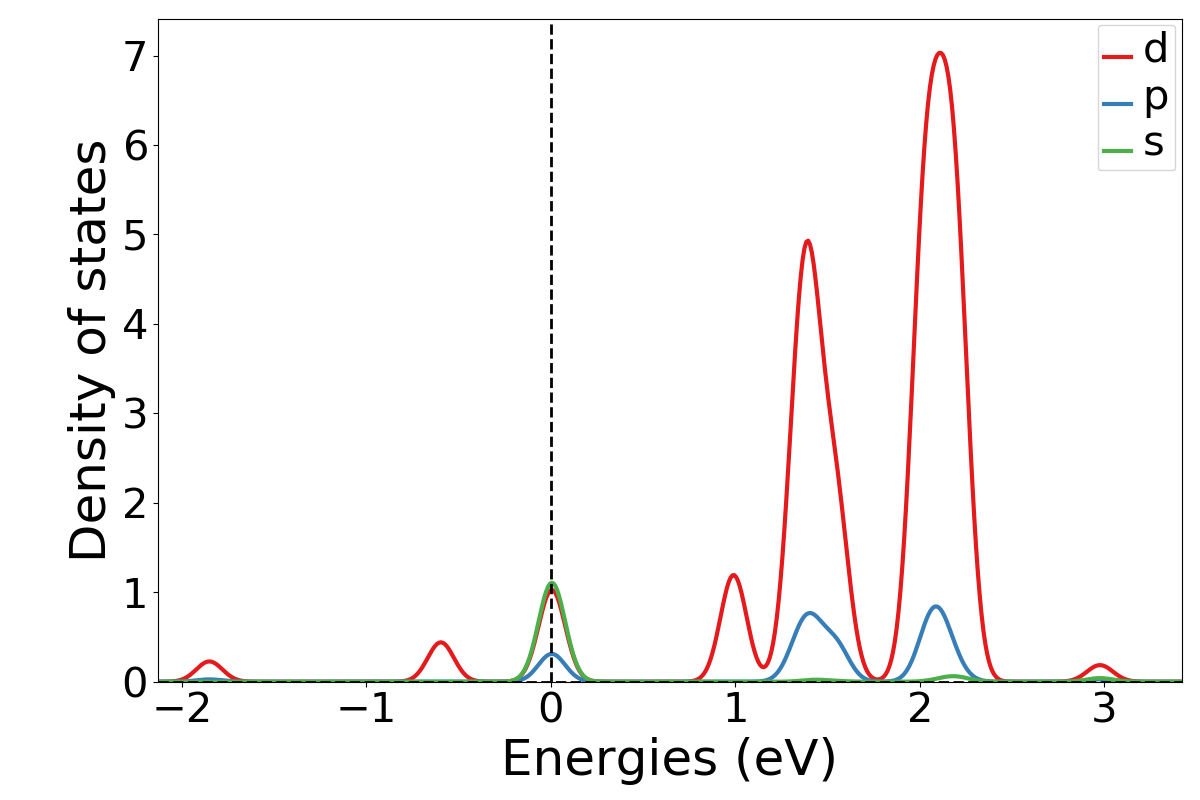
\includegraphics[width = 11cm]{../fig/Y_LDOS25_2.png}
        \caption{Plot of local DOS of atom number 25(Y in lower alcohol-group) for Quinizarin with Yttrium, zoomed in for energies between 0.0 eV and 4.5 eV. }
        \label{fig:Y_LDOS25_2.png}
      \end{figure}

      \begin{figure}[H]
        \centering
        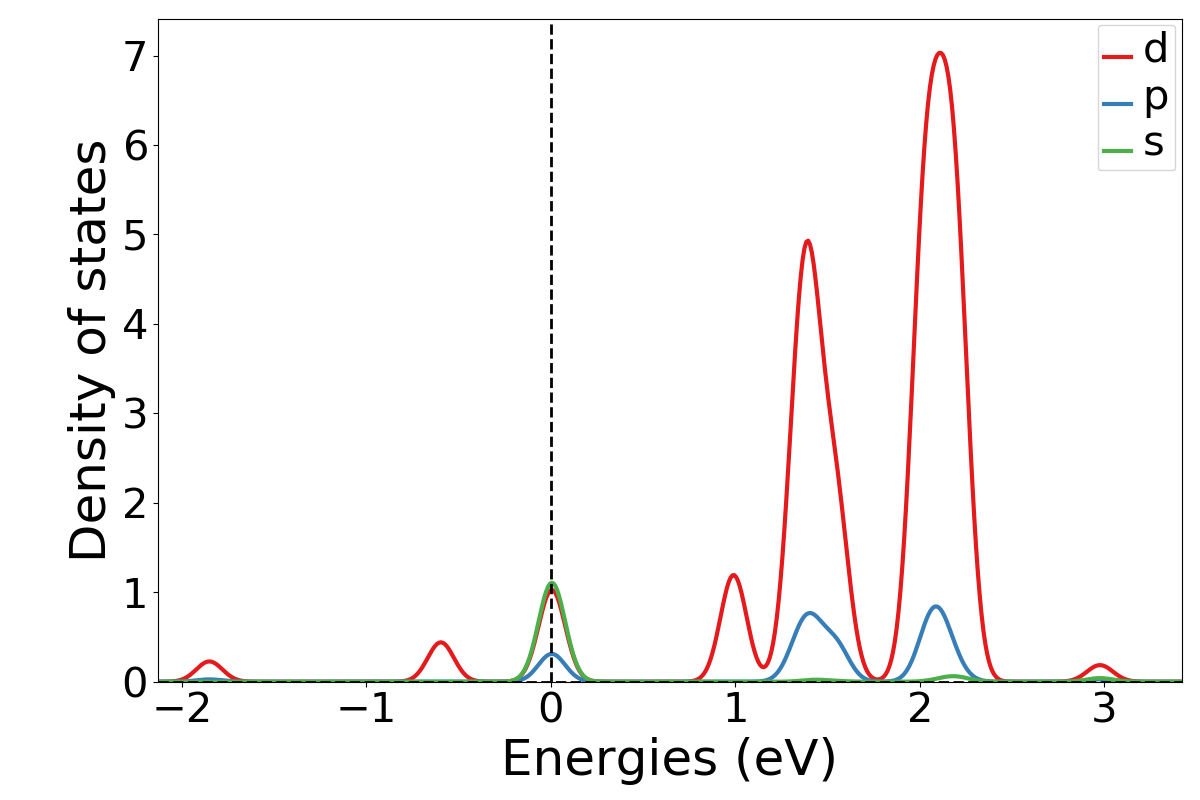
\includegraphics[width = 11cm]{../fig/Y_LDOS25_2.png}
        \caption{Plot of local DOS of atom number 25(Y in lower alcohol-group) for Quinizarin with Yttrium, zoomed in for energies between 0.0 eV and 4.5 eV. }
        \label{fig:Y_LDOS25_2.png}
      \end{figure}

      \begin{figure}[H]
          \centering
          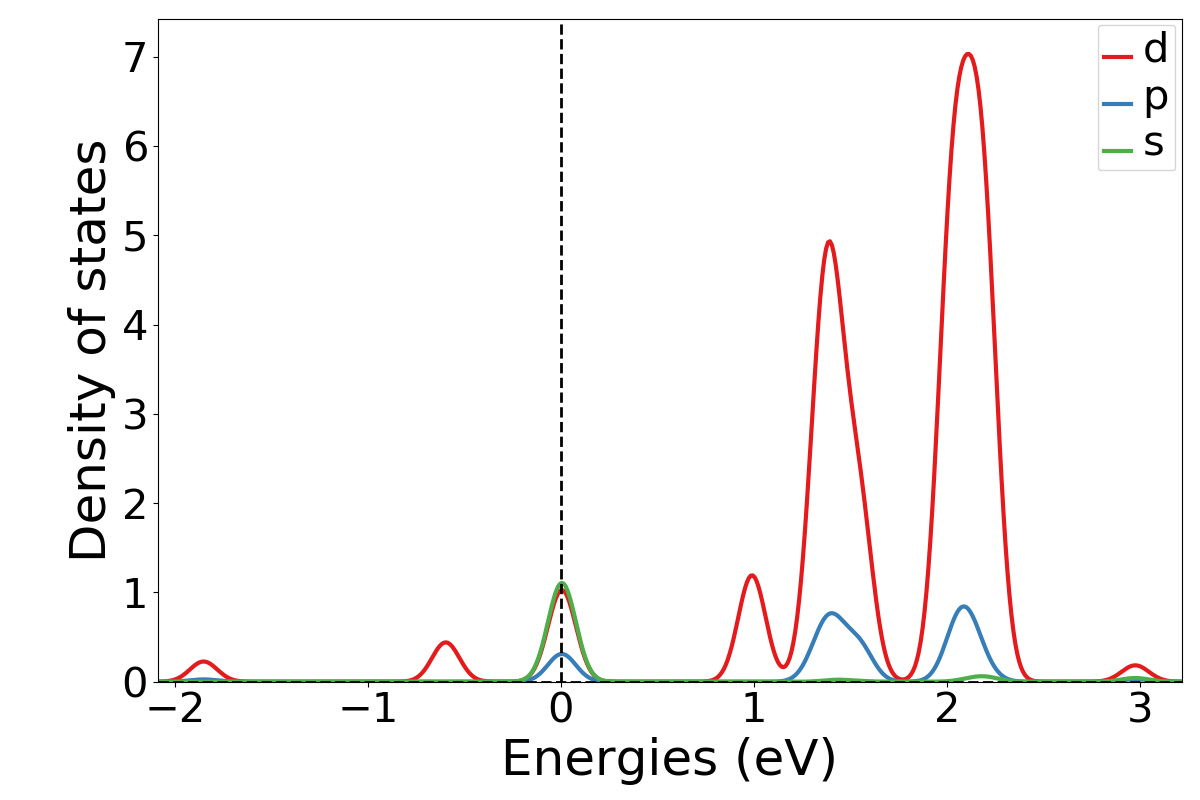
\includegraphics[width = 11cm]{../fig/Y_LDOS26_2.png}
          \caption{Plot of local DOS of atom number 26(Y in upper alcohol-group) for Quinizarin with Yttrium, zoomed in for energies between 0.0 eV and 4.5 eV. }
          \label{fig:Y_LDOS26_2.png}
      \end{figure}


    \subsubsection{Band gap}

      "The band gap was X eV"

      \begin{table}[H]
        \centering
        \caption{Band gap, valance band maximum and conduction band minimum for Quinizarin with Yttrium with static calculations. }
        \vspace{0mm}
        \label{tab:bandgapY}
        \begin{tabular}{|c|c|c|c|}
            \hline
            Calculation & Band gap [eV] & VBM [eV] & CBM [eV]  \\
            \hline \hline
            Before relax & $0.042$ & $-3.323$ & $-3.281$ \\
            After relax & $0.029$ & $-2.979$ & $-2.950$ \\
            \hline
        \end{tabular} \\
        \hspace{0pt}\\
      \end{table}

    \subsubsection{Charge density}

      Show CHGCAR figures

      \begin{figure}[H]
        \centering
        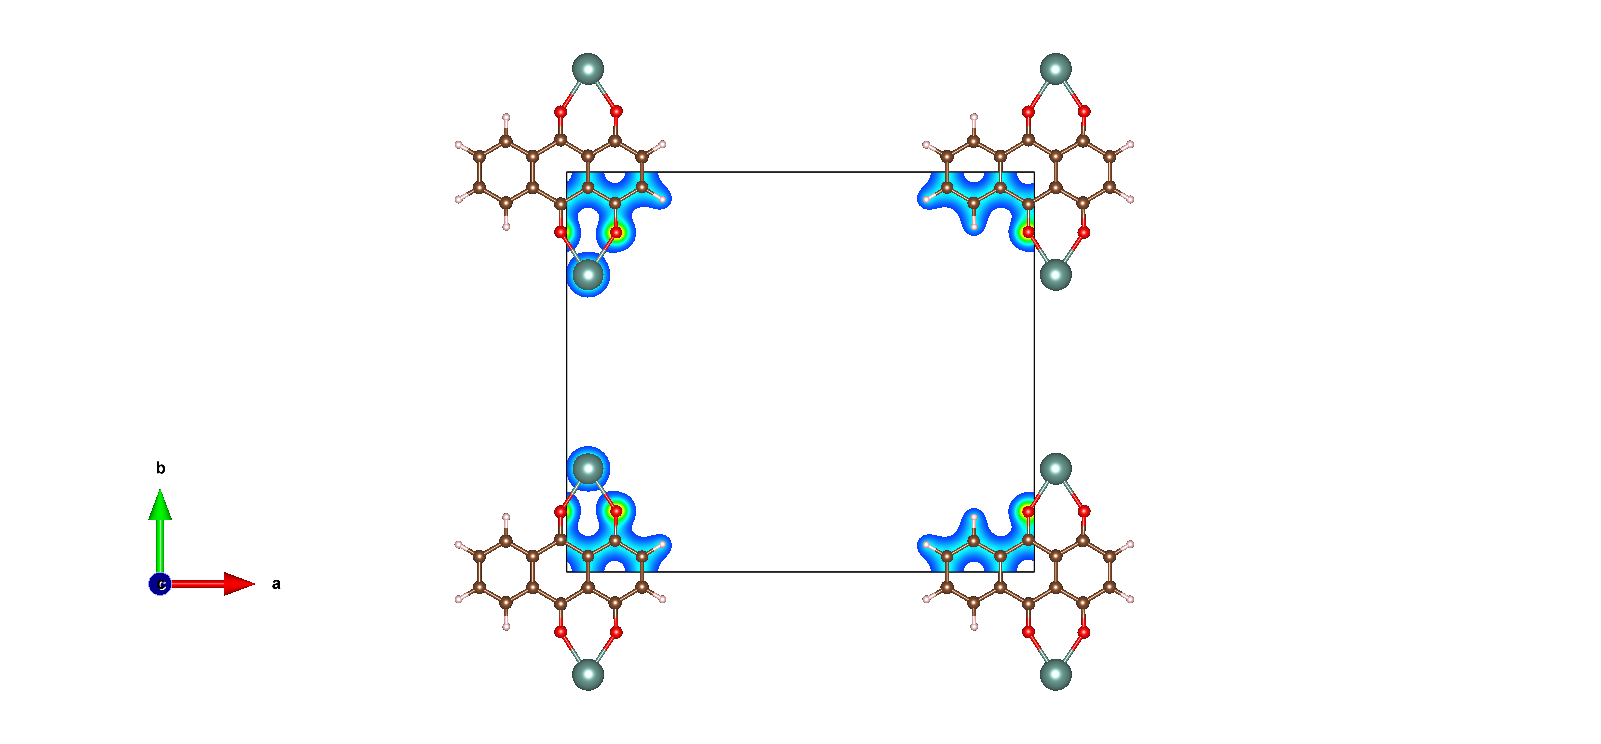
\includegraphics[width = 11cm]{../fig/Y_staticbefore_CHGCAR.png}
        \caption{Charge density of Quinizarin with Yttrium for static VASP calculation. }
        \label{fig:Y_staticbefore_CHGCAR}
      \end{figure}

      \begin{figure}[H]
        \centering
        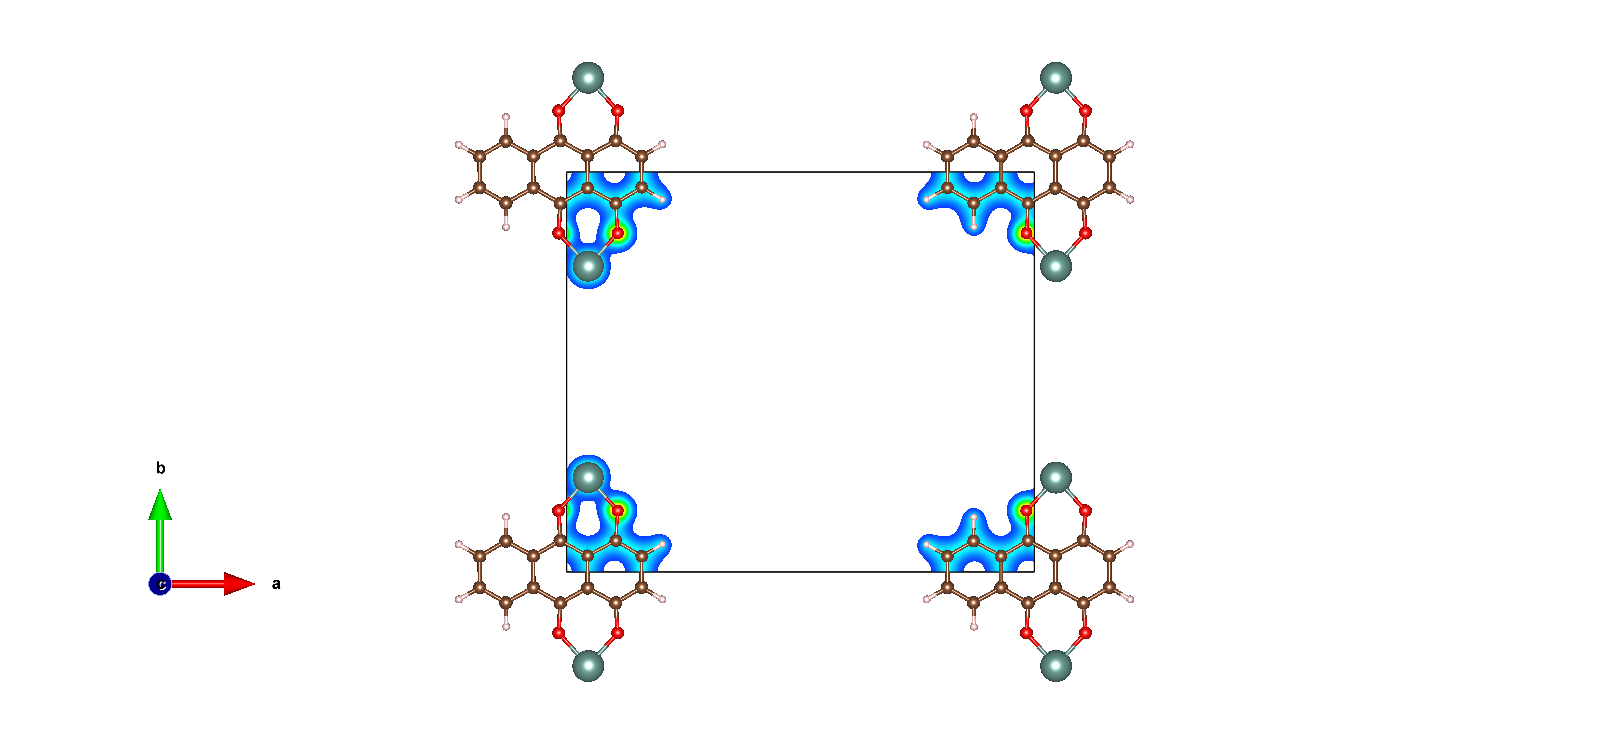
\includegraphics[width = 11cm]{../fig/Y_staticafter_CHGCAR.png}
        \caption{Charge density of Quinizarin with Yttrium for static VASP calculation after relaxed calculation. }
        \label{fig:Y_staticafter_CHGCAR}
      \end{figure}


  \subsection{Quinizarin with Ytterbium}

    \subsubsection{Relaxing the structure}

      Quinizarin with Ytterbium before relaxation is shown in Figure~(\ref{fig:Yb_staticbefore_CONTCAR}). After relaxation the structure looked as in Figure~(\ref{fig:Yb_staticafter_CONTCAR}).

      \begin{figure}[H]
        \centering
        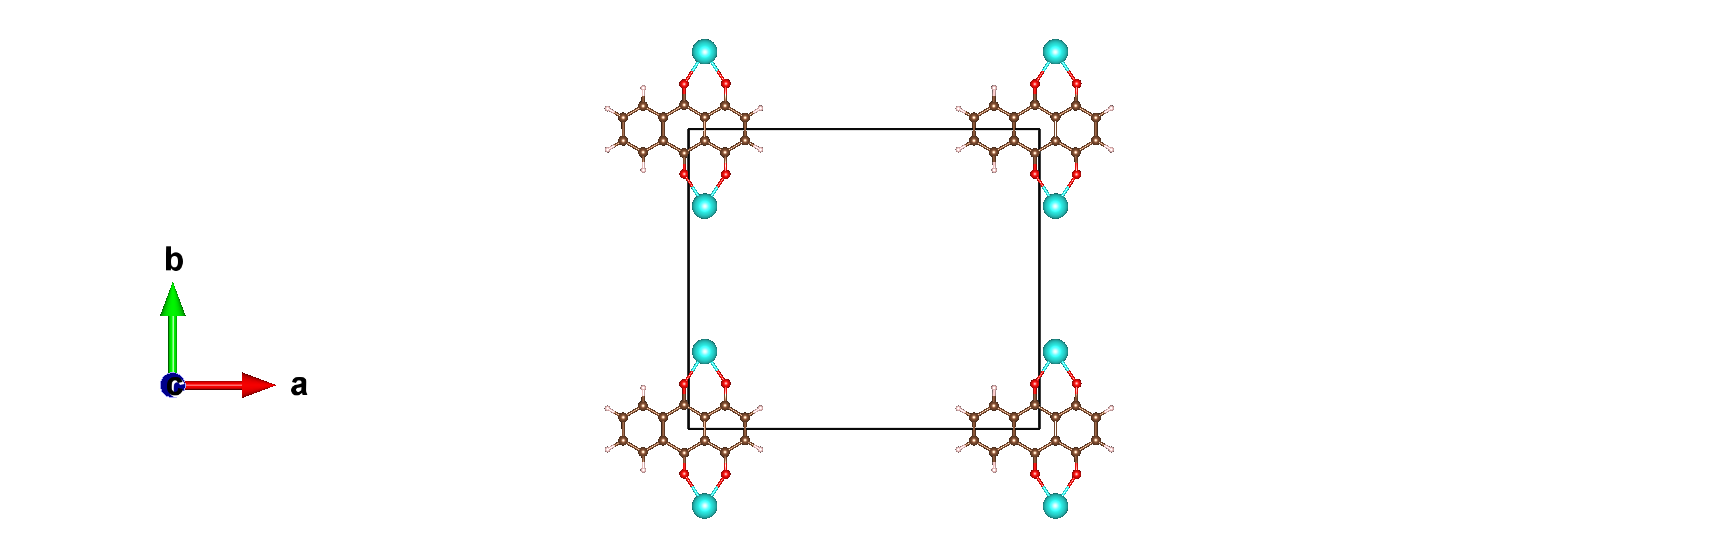
\includegraphics[width = 11cm]{../fig/Yb_staticbefore_CONTCAR.png}
        \caption{Structure of Quinizarin with Ytterbium for static VASP calculation. }
        \label{fig:Yb_staticbefore_CONTCAR}
      \end{figure}

      \begin{figure}[H]
        \centering
        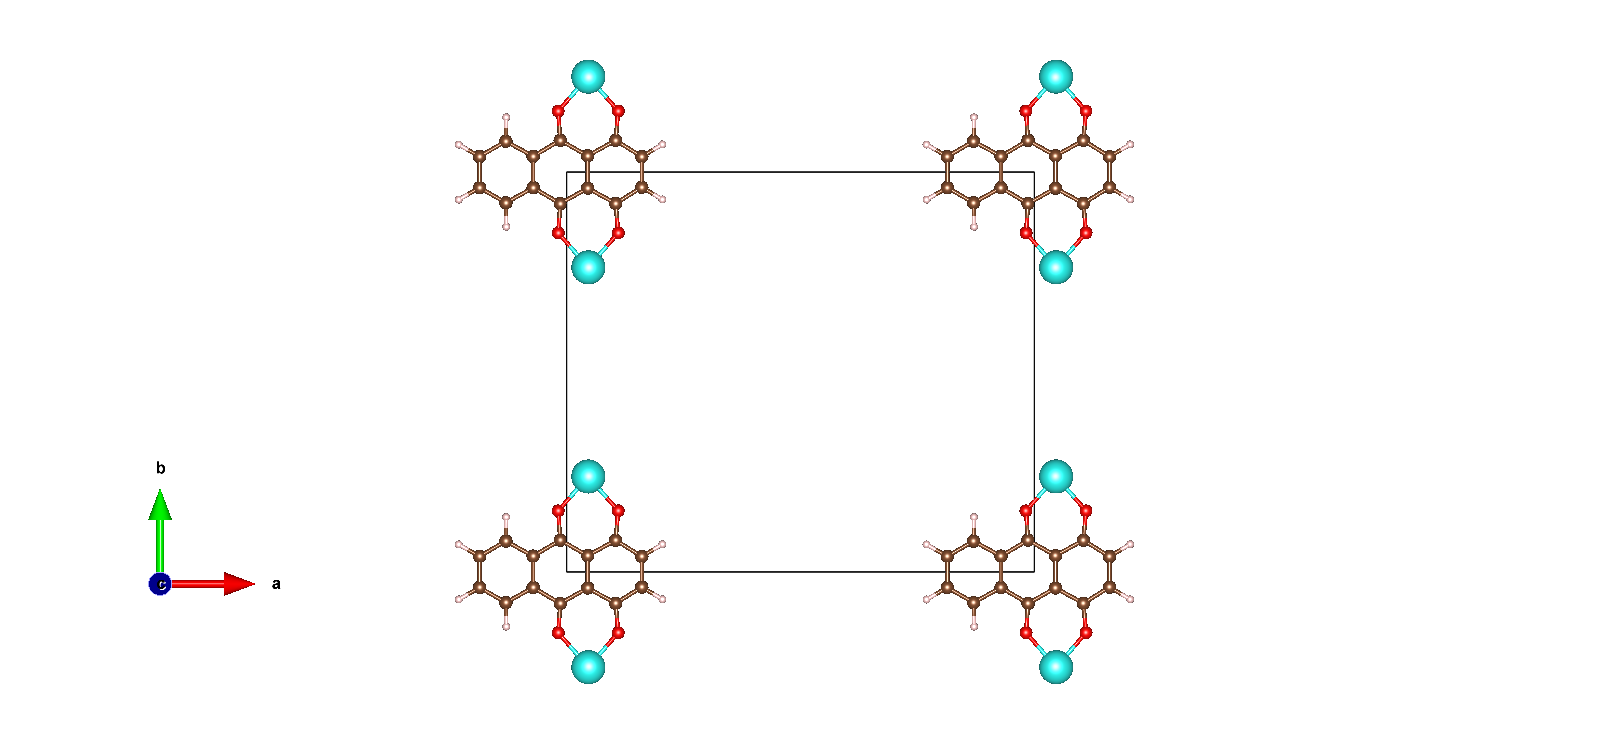
\includegraphics[width = 11cm]{../fig/Yb_staticafter_CONTCAR.png}
        \caption{Structure of Quinizarin with Ytterbium for static VASP calculation after relaxed calculation. }
        \label{fig:Yb_staticafter_CONTCAR}
      \end{figure}

    \subsubsection{Total and relative energies}

      See Table~(\ref{tab:TOTENYb}) for a table comparing the total energies of the VASP calculations of Quinizarin with Ytterbium. The relative energy was 0.013 eV difference.

      \begin{table}[H]
        \centering
        \caption{Total energy per atom for Quinizarin with Ytterbium before and after relaxation. }
        \label{tab:TOTENYb}
        \begin{tabular}{|c|c|}
            \hline
            Calculation & Total energy per atom [eV/atom]  \\
            \hline \hline
            Before relax & $-6.869$ \\
            After relax & $-6.882$ \\
            \hline
        \end{tabular} \\
        \hspace{0pt}\\
      \end{table}

    \subsubsection{Total and Local density of states}

      TDOS and LDOS graphs


      \begin{figure}[H]
        \centering
        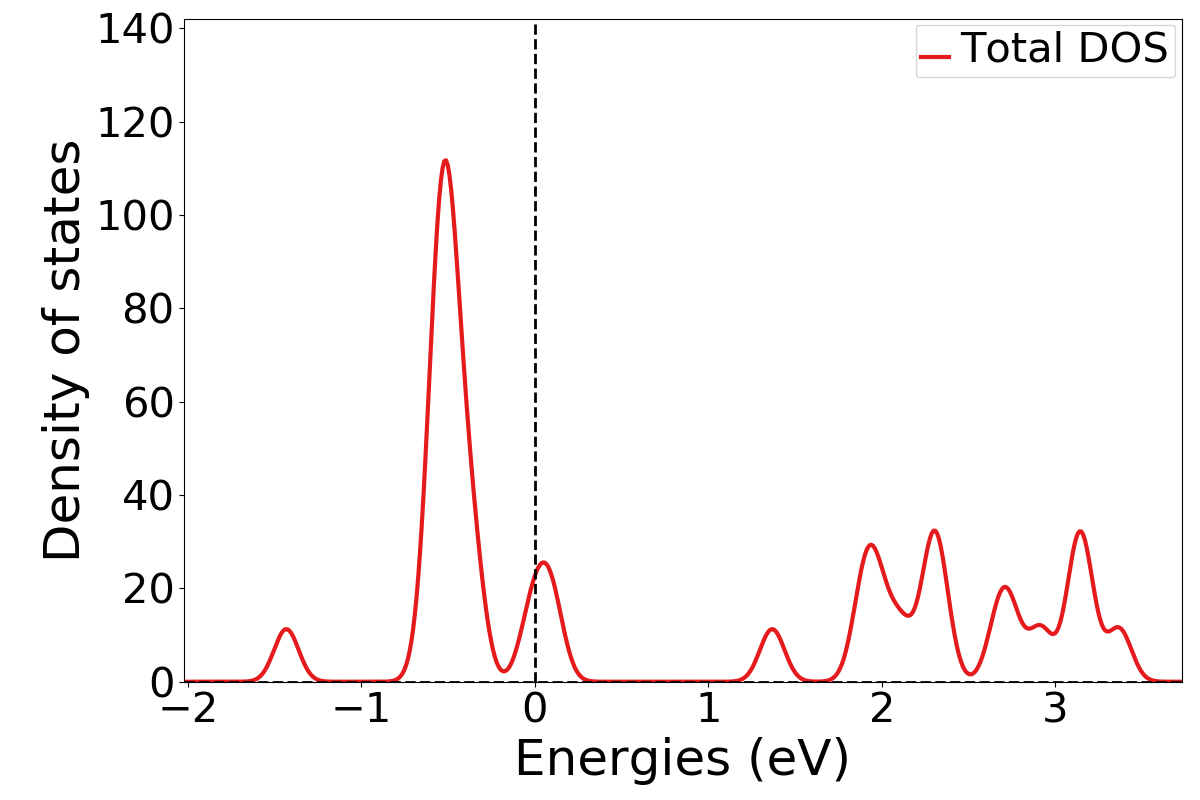
\includegraphics[width = 11cm]{../fig/Yb_TDOS_2.png}
        \caption{Plot of total DOS for Ytterbium, zoomed in for energies between 0.0 eV and 8.0 eV. }
        \label{fig:Yb_TDOS_2.png}
      \end{figure}

      \begin{figure}[H]
          \centering
          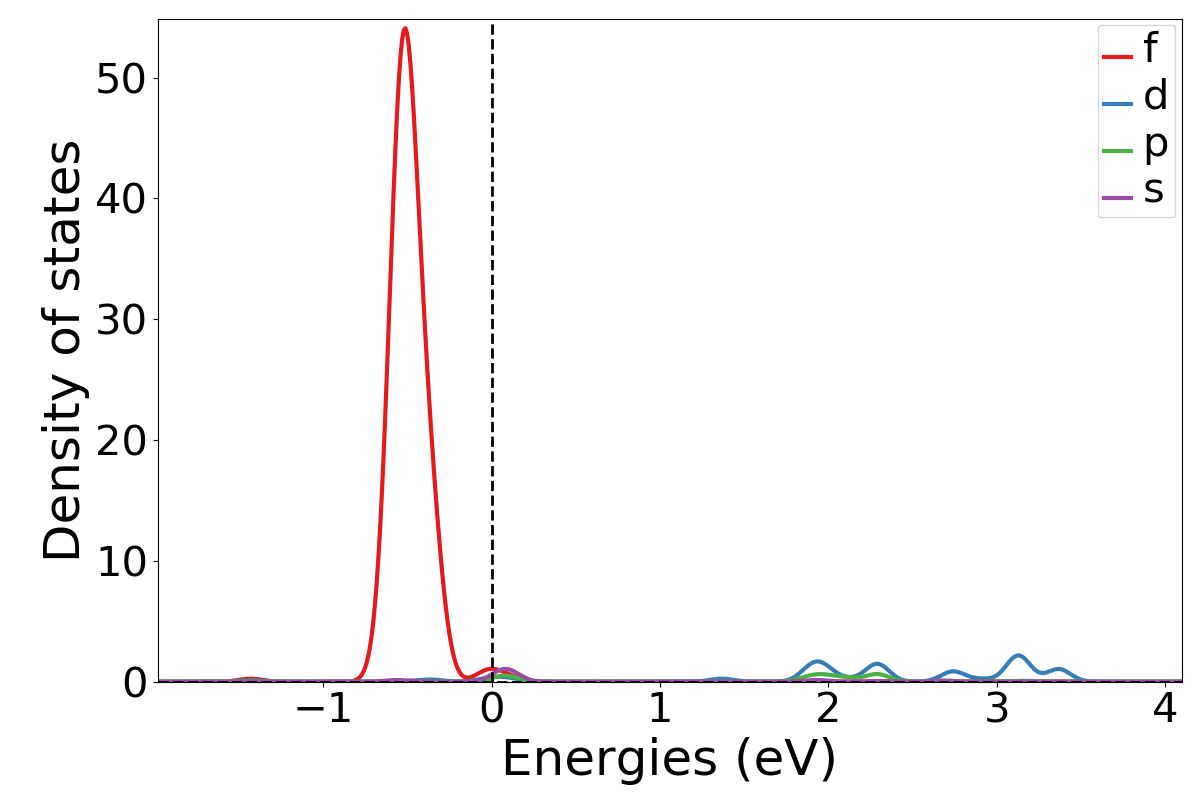
\includegraphics[width = 11cm]{../fig/Yb_LDOS25_2.png}
          \caption{Plot of local DOS of atom number 25(Yb in lower alcohol-group) for Quinizarin with Ytterbium, zoomed in for energies between 0.0 eV and 8.0 eV. }
          \label{fig:Yb_LDOS25_2.png}
      \end{figure}

      \begin{figure}[H]
          \centering
          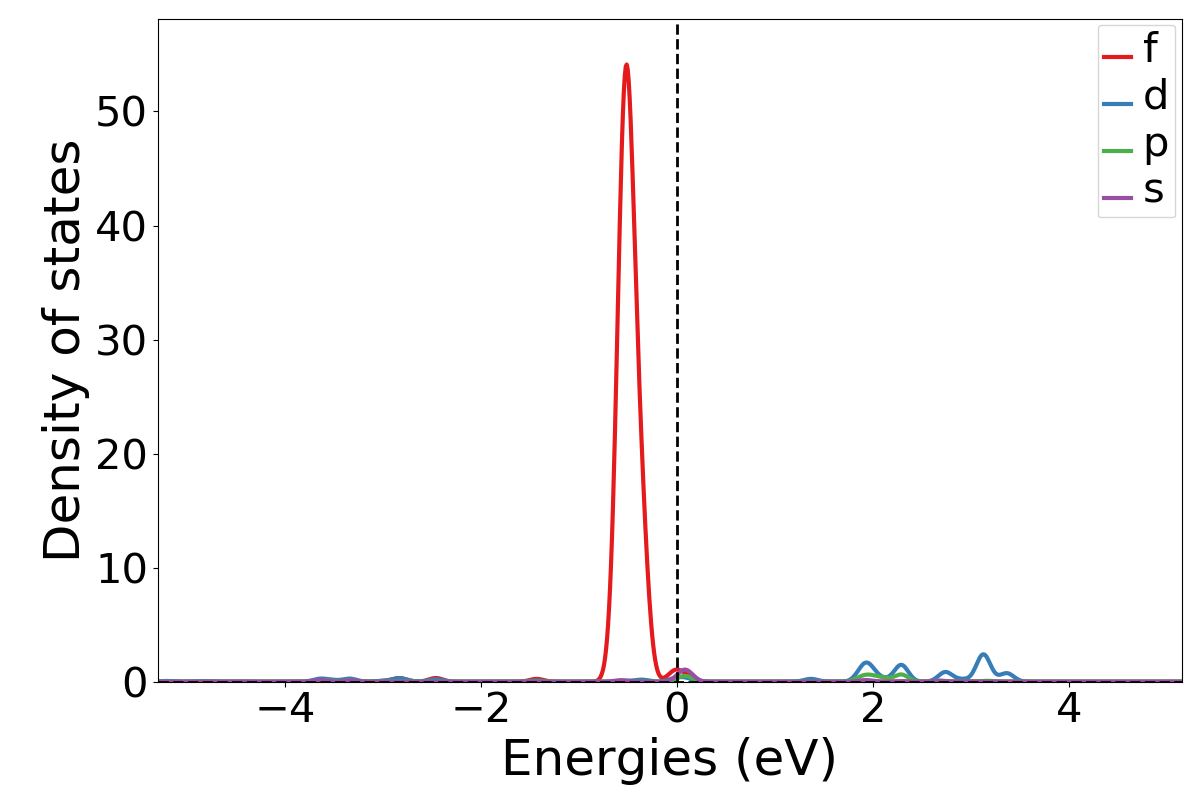
\includegraphics[width = 11cm]{../fig/Yb_LDOS26_2.png}
          \caption{Plot of local DOS of atom number 26(Yb in upper alcohol-group) for Quinizarin with Ytterbium, zoomed in for energies between 0.0 eV and 8.0 eV. }
          \label{fig:Yb_LDOS26_2.png}
      \end{figure}



    \subsubsection{Band Gaps}

      "The band gap was X eV"

      \begin{table}[H]
        \centering
        \caption{Band gap, valance band maximum and conduction band minimum for Quinizarin with Ytterbium with static calculations. }
        \vspace{0mm}
        \label{tab:bandgapYb}
        \begin{tabular}{|c|c|c|c|}
            \hline
            Calculation & Band gap [eV] & VBM [eV] & CBM [eV]  \\
            \hline \hline
            Before relax & $0.0552$ & $-2.9157$ & $-2.6422$ \\
            After relax & $0.0771$ & $-2.7193$ & $-3.720$ \\
            \hline
        \end{tabular} \\
        \hspace{0pt}\\
      \end{table}

    \subsubsection{Charge Density}

      Show CHGCAR figures

  \subsection{Quinizarin with Neodymium}




\vspace{1cm}

\section{Discussion}    \label{sec:Discussion}

  \subsection{Convergence of energy}

    Figure~(\ref{fig:convergence_energy.png}) shows that the values change quite rapidly and reach a peak around cutoff 500 eV which then loweres and stabilizes near cutoff 800 eV. However, the values differ by a very small amount, which can indicate that one needs a smaller cuttoff energy than 800. Figure~(\ref{fig:convergence_energy_difference.png}) also indicates this. \\

    From Section~\ref{sec:Convergence} we learned that if the difference in energy is less than 0.003 eV the calculation can be considered converged. The figure shows that ENCUT=450 is below 0.002 eV in difference from ENCUT=500. This shows that ENCUT=450 is safe enough to use. This can seem weird due to it being before a peak and the stabilized total energy is lower, but the values are quite small, and overall should not impact the results in a meaningful way. \\

  \subsection{Convergence of k-points}

    There were fewer data points than with the energy convergence, so it is not as easy to find a pattern as it was with the convergence of energy. For Figure~(\ref{fig:convergence_kpoints.png}) one can see the energy increases to a peak around 4.0 and 5.0 in k-density, which then decreases at k-density 6.0. Due to the lack of a good pattern we quickly moved on to Figure~(\ref{fig:convergence_kpoints_difference.png}) which showed even less of a converging pattern. However, already at k-density 1.0 we could see the difference was less than 0.003 eV. Since the difference increased again with 2.0, we wondered if we could use 3.0, but after a few test-calculations with both 1.0 and 3.0 we found the difference was negligible and so we chose to use 1.0. \\


  \subsection{Quinizarin}


  \subsection{Quinizarin with Yttrium}


  \subsection{Quinizarin with Ytterbium}


  \subsection{Quinizarin with Neodymium}


  \subsection{Total comparison}




\vspace{1cm}

\section{Conclusion}    \label{sec:Conclusion}


%--------------------- References --------------------------------------------
\vspace{1cm}

\section{References} \label{sec:References}

    \begin{thebibliography}{}

    \bibitem{laereboken}
    Ben G. Streetman \& Sanjay Kumar Banerjee, 2016, \textit{Solid State Elctronic Devices seventh edition}, Pearson Education


    \end{thebibliography}


%------------------ Appendix ------------------------------------

\appendix  \label{sec:Appendix}

\iffalse

\section{Quinizarin-bilder}



  \begin{figure}[H]
      \centering
      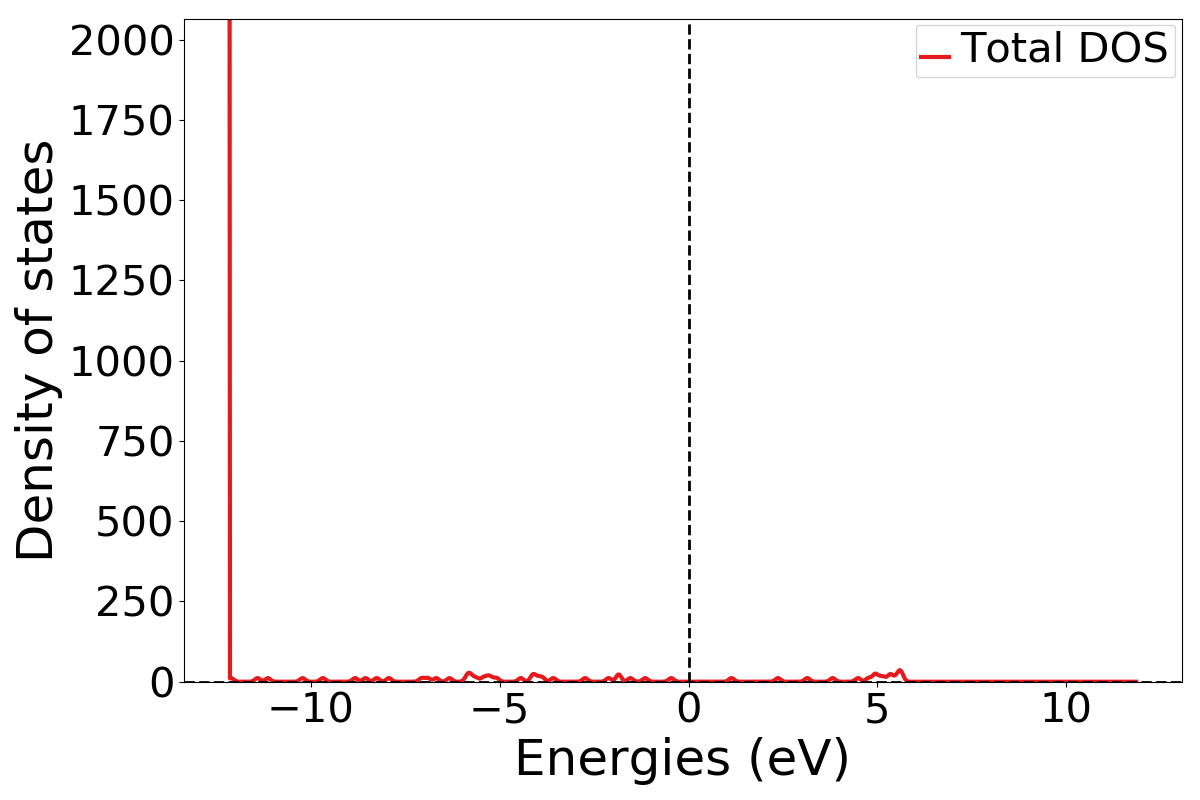
\includegraphics[width = 11cm]{../fig/basic_TDOS_1.png}
      \caption{Plot of total DOS for Quinizarin. }
      \label{fig:basic_TDOS_1}
  \end{figure}

  \begin{figure}[H]
      \centering
      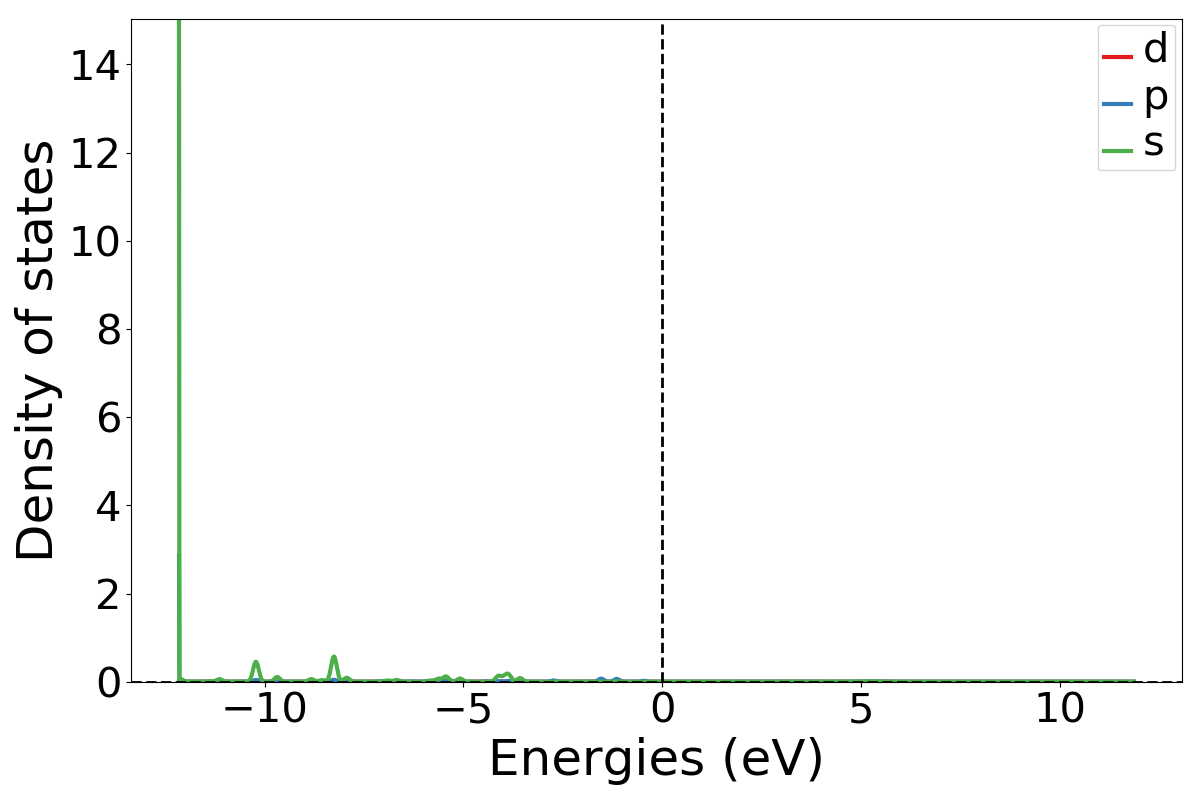
\includegraphics[width = 11cm]{../fig/basic_LDOS25_1.png}
      \caption{Plot of local DOS for atom number 25(H in alcohol-group) for Quinizarin.}
      \label{fig:basic_LDOS25_1}
  \end{figure}

  \begin{figure}[H]
      \centering
      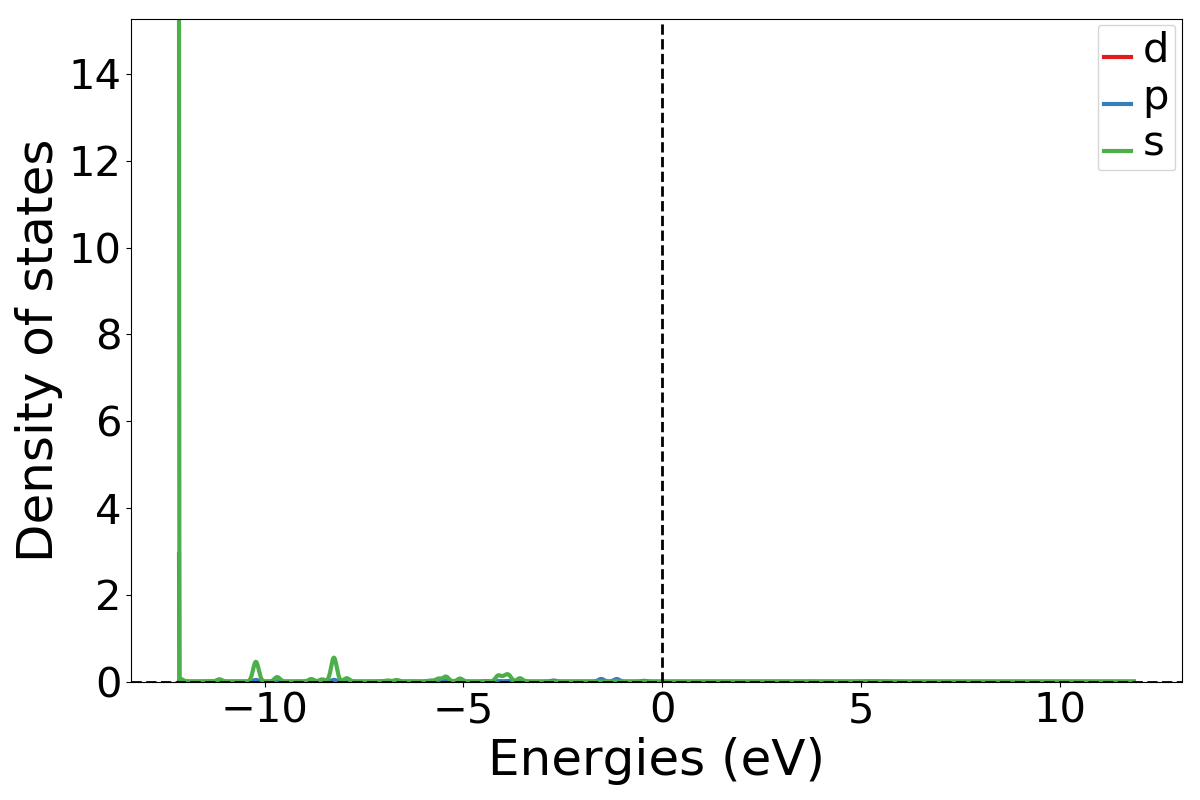
\includegraphics[width = 11cm]{../fig/basic_LDOS26_1.png}
      \caption{Plot of local DOS for atom number 26(H in alcohol-group) for Quinizarin. }
      \label{fig:basic_LDOS26_1}
  \end{figure}

\vspace{1cm}

\section{Y-bilder}


  \begin{figure}[H]
      \centering
      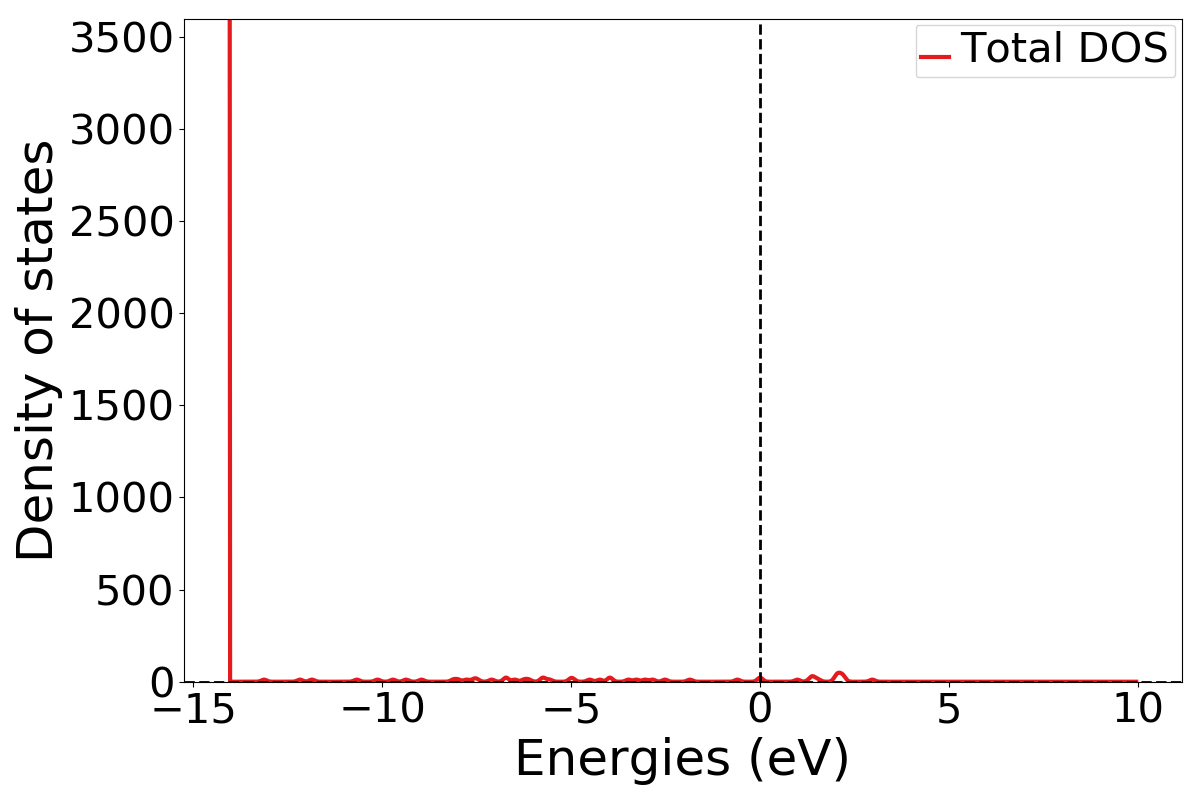
\includegraphics[width = 11cm]{../fig/Y_TDOS_1.png}
      \caption{Plot of total DOS for Quinizarin with Yttrium. }
      \label{fig:Y_TDOS_1.png}
  \end{figure}

  \begin{figure}[H]
      \centering
      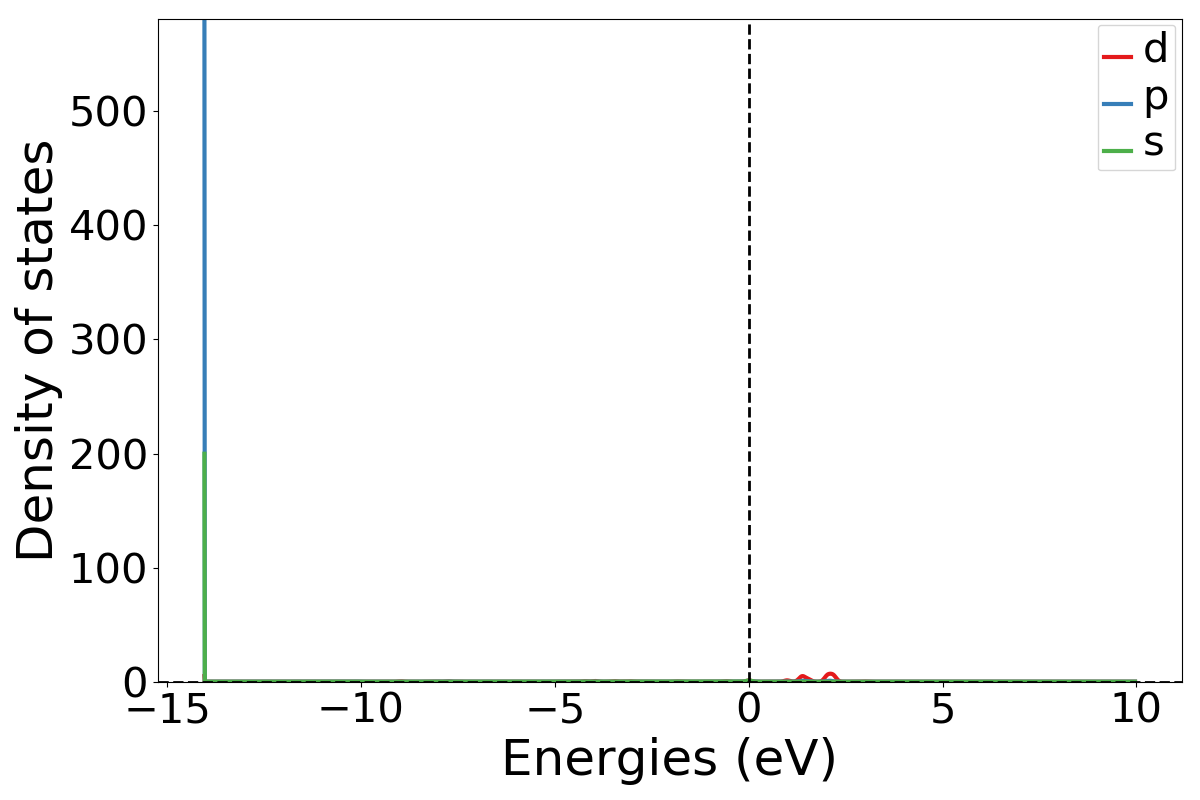
\includegraphics[width = 11cm]{../fig/Y_LDOS25_1.png}
      \caption{Plot of local DOS of atom number 25(Y in lower alcohol-group) for Quinizarin with Yttrium. }
      \label{fig:Y_LDOS25_1.png}
  \end{figure}

  \begin{figure}[H]
      \centering
      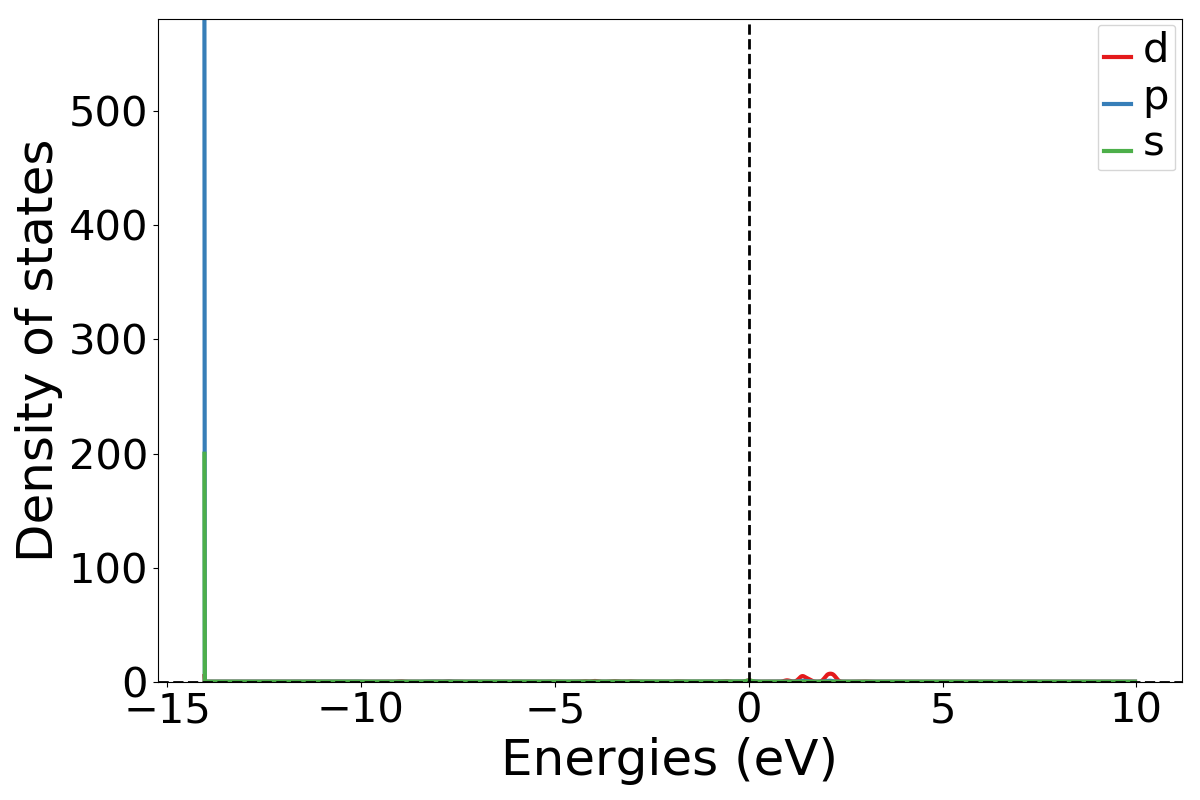
\includegraphics[width = 11cm]{../fig/Y_LDOS26_1.png}
      \caption{Plot of local DOS of atom number 26(Y in upper alcohol-group) for Quinizarin with Yttrium. }
      \label{fig:Y_LDOS26_1.png}
  \end{figure}

\vspace{1cm}

\section{Yb-bilder}



  \begin{figure}[H]
      \centering
      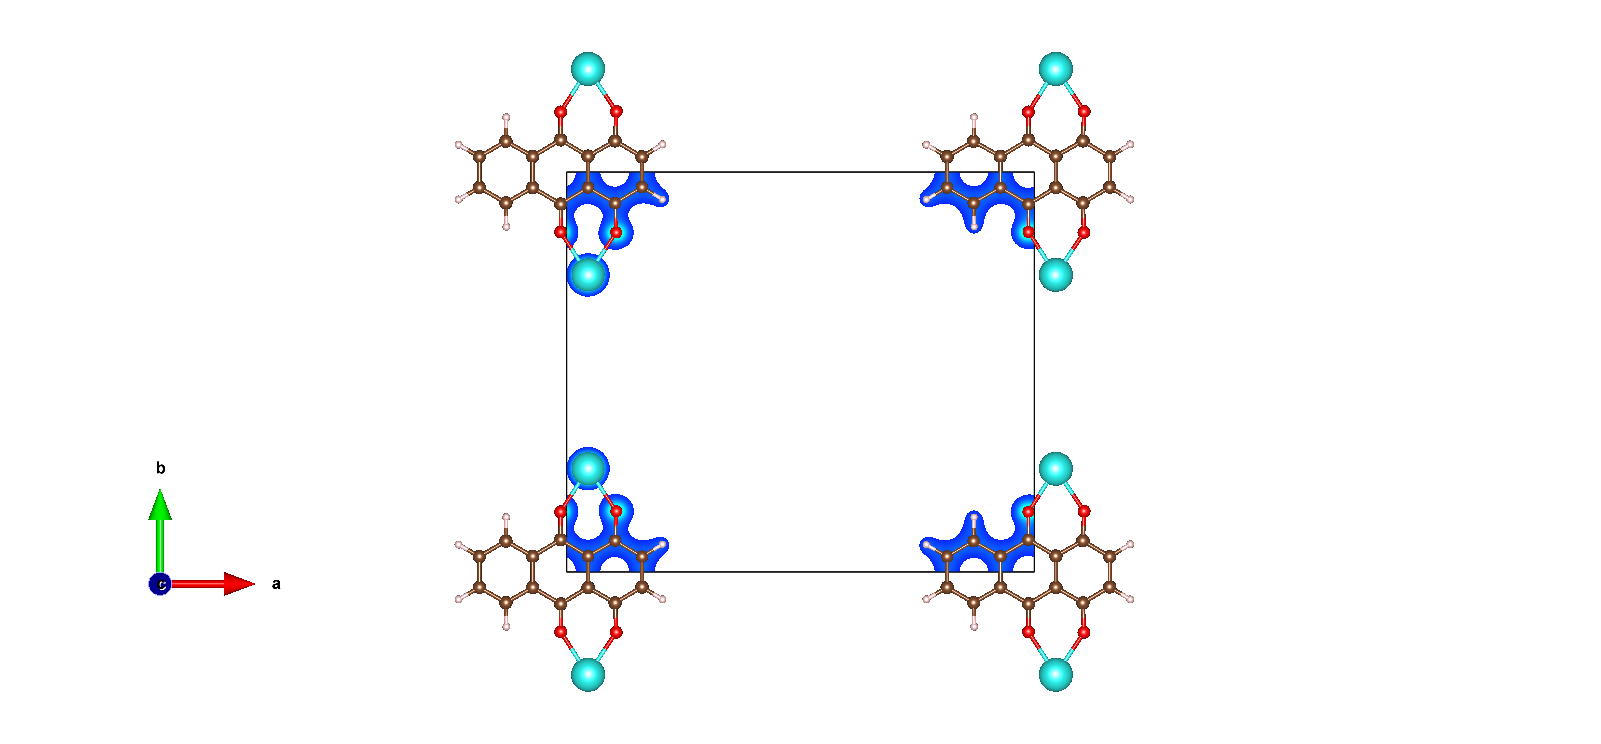
\includegraphics[width = 11cm]{../fig/Yb_staticbefore_CHGCAR.png}
      \caption{Charge density of Quinizarin with Ytterbium for static VASP calculation. }
      \label{fig:Yb_staticbefore_CHGCAR}
  \end{figure}


  \begin{figure}[H]
      \centering
      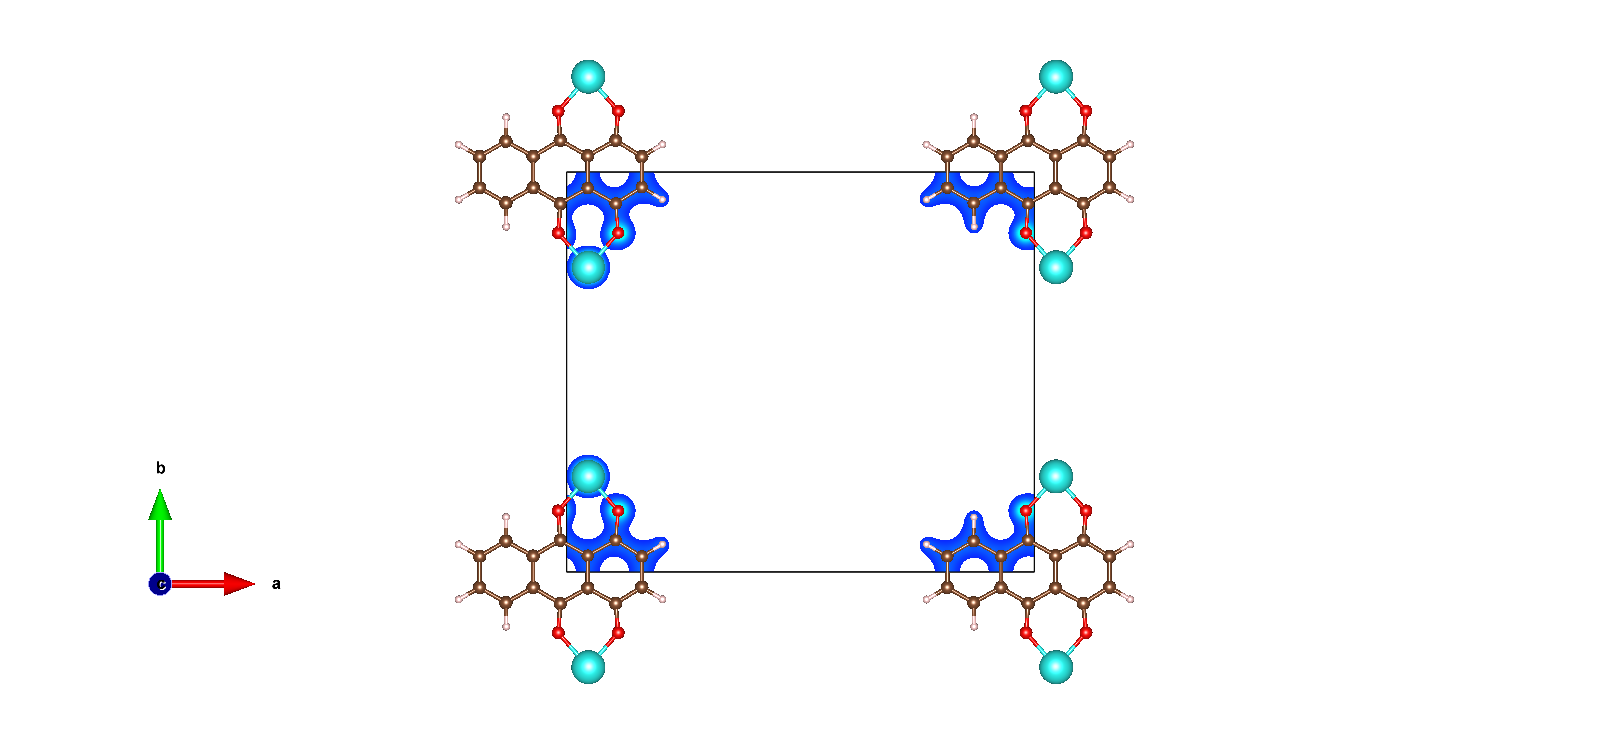
\includegraphics[width = 11cm]{../fig/Yb_staticafter_CHGCAR.png}
      \caption{Charge density of Quinizarin with Ytterbium for static VASP calculation after relaxed calculation. }
      \label{fig:Yb_staticafter_CHGCAR}
  \end{figure}

  \begin{figure}[H]
      \centering
      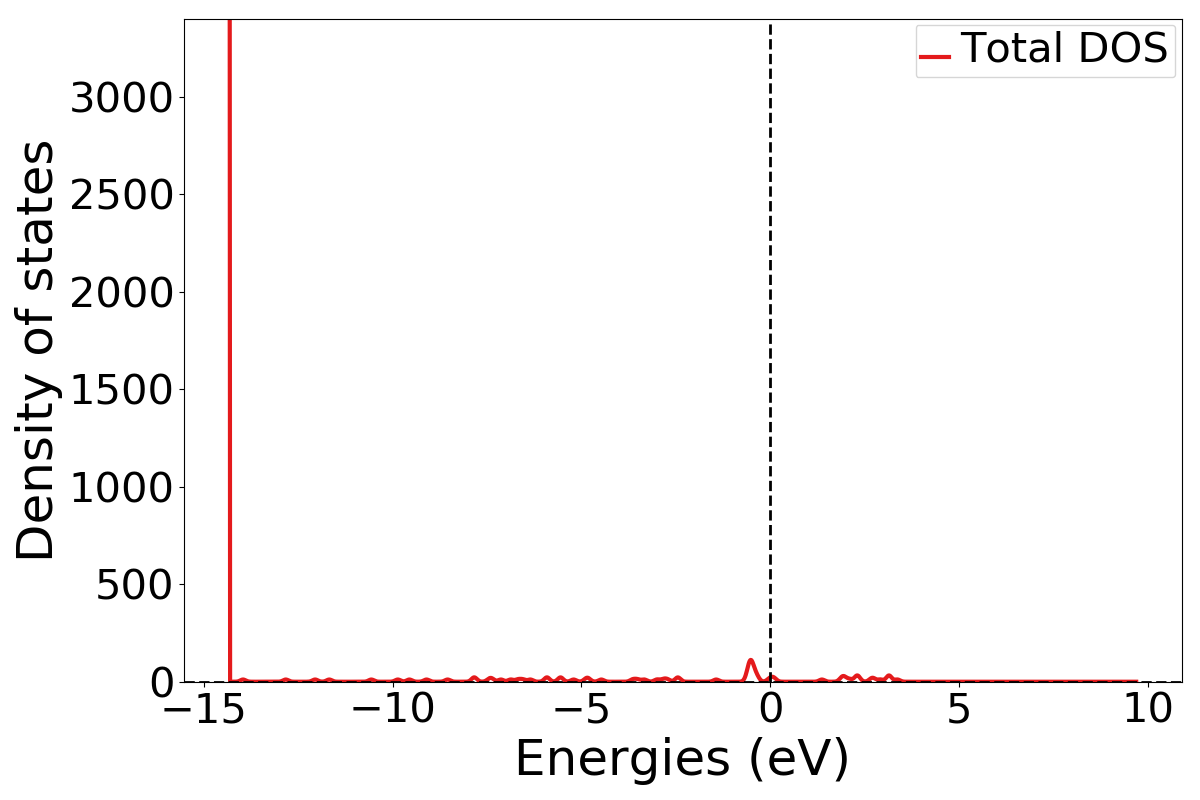
\includegraphics[width = 11cm]{../fig/Yb_TDOS_1.png}
      \caption{Plot of total DOS for Ytterbium. }
      \label{fig:Yb_TDOS_1.png}
  \end{figure}

  \begin{figure}[H]
      \centering
      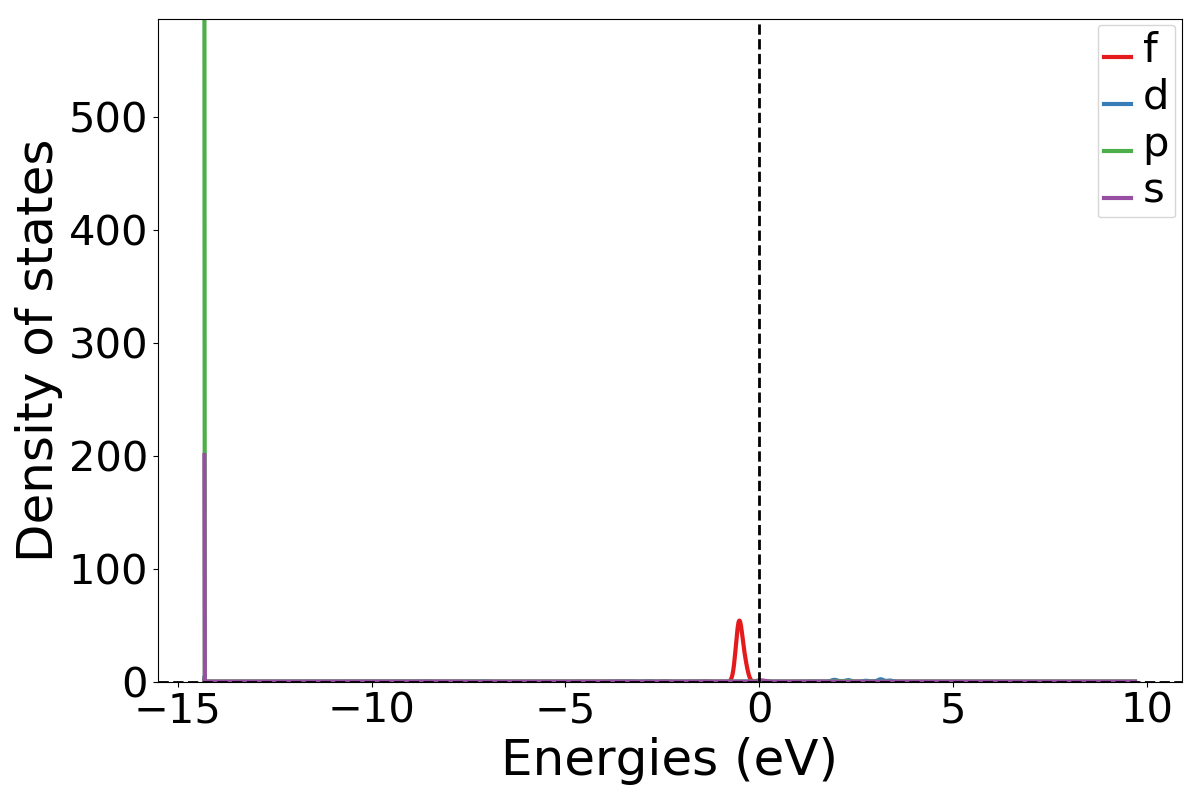
\includegraphics[width = 11cm]{../fig/Yb_LDOS25_1.png}
      \caption{Plot of local DOS of atom number 25(Yb in lower alcohol-group) for Quinizarin with Ytterbium. }
      \label{fig:Yb_LDOS25_1.png}
  \end{figure}

  \begin{figure}[H]
      \centering
      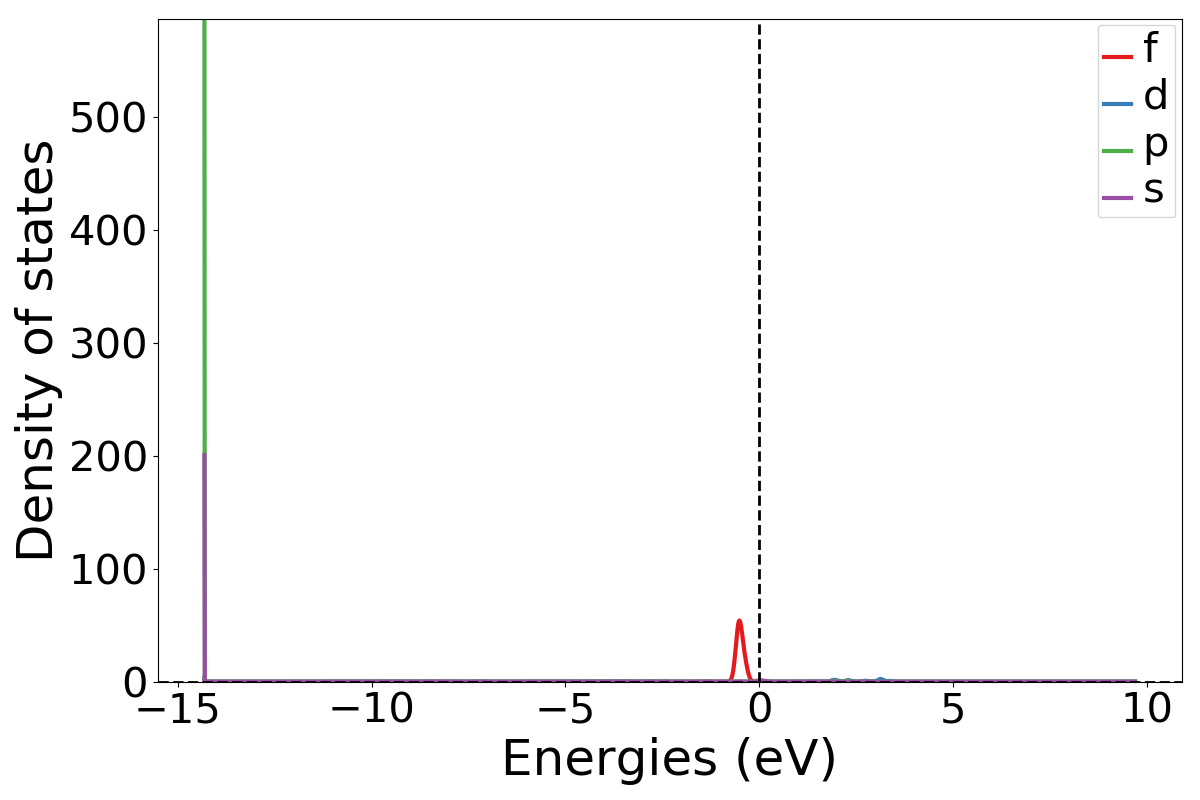
\includegraphics[width = 11cm]{../fig/Yb_LDOS26_1.png}
      \caption{Plot of local DOS of atom number 26(Yb in upper alcohol-group) for Quinizarin with Ytterbium. }
      \label{fig:Yb_LDOS26_1.png}
  \end{figure}

\fi

\vspace{1cm}

\section{Appendix 1}

    \iffalse
    \begin{python}
        import numpy as np

        N = 100

        x = np.linspace(1, 100, N)

        def f(x):
            return x**2

        y = f(x)

        print(y)


        test for cpp, men er nok bedre med den andre versjonen med lstlisting

        std::cout << "index, value\n";
      for(int i = 0; i < n; i++){
          std::cout << "    " << i << ", " << d_new[i] << std::endl;
      }

    \end{python}

    \begin{lstlisting}[language = python] — må huske å ha den ekstra delen til farger osv.
    \end{lstlisting}
    \fi

    \iffalse
    \begin{figure}[H]
        \centering
            \begin{tikzpicture}
            \draw[black, thick, ->] (-3,0) -- (4,0) node[anchor=west] {$x$};
            \draw[black, thick, ->] (0,-3) -- (0,3) node[anchor=south] {$\rho(x)$};
            \draw[cyan, thick, |-|, densely dashed] (-0.2,2.3) -- (3,2.3) ;
            \draw[cyan] (1.8,2.3) circle [radius = 0.01pt] node[anchor= south east] {$W$};
            \draw[thick] (0,0)--(0,2)--(3,2)--(3,0)--(0,0);
            \draw[text=cyan] (1,1.2)  node[anchor=north west] {$Q_s$};
            \fill[black] (3,0) circle [radius = 1.5pt] ;
            \draw[text=cyan] (3,0) node[anchor = north] {$x_{n0}$};
            \draw[thick] (0,0)--(0,-2)--(-0.2,-2)--(-0.2,0)--(0,0);
            \draw[text=cyan] (-1,-1)  node[anchor=north west] {$Q_m$};
            \fill[black] (-0.2,0) circle [radius = 1.5pt] ;
            \draw[text=cyan] (-0.2,0) node[anchor = south east] {$x_{p0}$};
        \end{tikzpicture}
        \caption{Ladningstetthet i deplesjonssonen for Schottkyovergangen.}
        \label{fig:schottkyladningstetthet}
    \end{figure}

    \begin{figure}[H]
        \centering
        \resizebox{17cm}{11cm}{
            \begin{tikzpicture}
                \draw [blue, thick, decoration={markings, mark=at position 0.750 with {\arrow{>}}}, postaction={decorate}] (3,0) arc(0:180:3);
                \draw [blue, thick, decoration={markings, mark=at position 0.250 with {\Huge \arrow{>}}}, postaction={decorate}] (3,0) arc(0:180:3);
                \draw [red, thick, decoration={markings, mark=at position 0.250 with {\arrow{<}}}, postaction={decorate}] (-1.10,0) arc(0:180:0.4cm);
                \draw [red, thick, decoration={markings, mark=at position 0.250 with {\arrow{<}}}, postaction={decorate}] (1.9,0) arc(0:180:0.4cm);
                \draw[text=blue] (0,3) node[anchor=north west] {$C_\rho$};
                \draw [->](-5,0) -- (5,0)  node[anchor=west] {$x$};
                \draw [->](0,-2) -- (0,5)  node[anchor=north east] {$y$};
                \fill[black] (3,0) circle [radius = 1.5pt] ;
                \draw [red, thick, decoration={markings, mark=at position 0.5 with {\arrow{>}}}, postaction={decorate}](-1.114,0) -- (1.114,0)  node[midway, anchor= south west] {$\gamma_\rho$};
                \draw [red, thick](-3,0) -- (-1.886,0);
                \draw [red, thick](3,0) -- (1.886,0);

                \fill[black] (3,0) circle [radius = 1.5pt] ;
                \draw[text=black] (3,0) node[anchor = north] {$1$};
                \fill[black] (-3,0) circle [radius = 1.5pt] ;
                \draw[text=black] (-3,0) node[anchor = north] {$-1$};
                \draw[black] (0,1.5) node[cross] {};
                \draw[text=black] (0,1.5) node[anchor = west] {$\frac{1}{2}i$};
                \draw[black] (-1.5,0) node[cross] {};
                \draw[text=black] (-1.5,0) node[anchor = north] {$-\frac{1}{2}$};
                \draw[black] (1.5,0) node[cross] {};
                \draw[text=black] (1.5,0) node[anchor = north] {$\frac{1}{2}$};
            \end{tikzpicture} }
        \caption{Konturen til integralet.}
        \label{fig:kontur}
    \end{figure}

    \begin{figure}[ht]
        \centering
        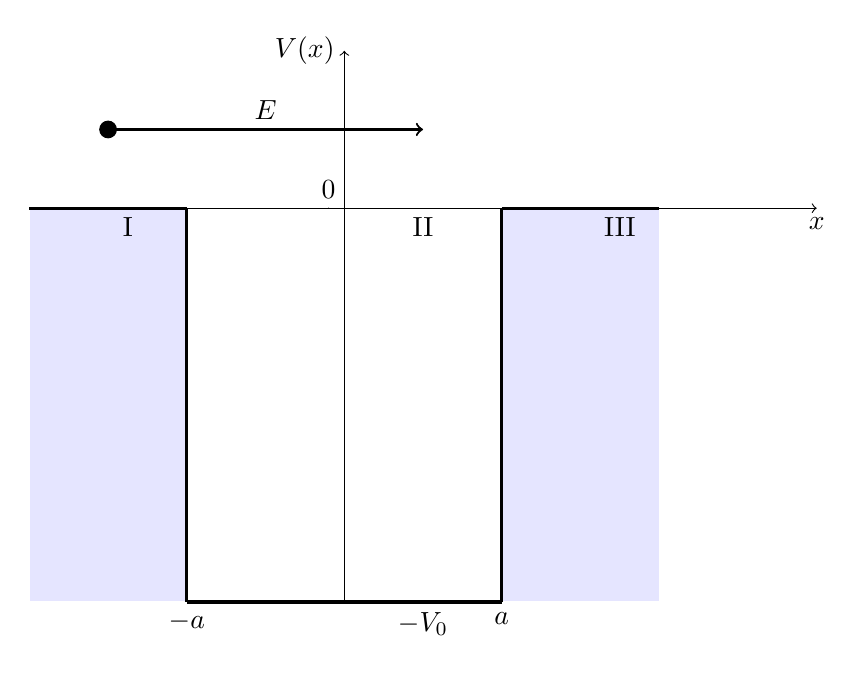
\begin{tikzpicture}
            \draw (-4,0) -- (-2,0);
            \draw (2,0) -- (4,0);
            \draw [fill = blue!10, draw = white] (-4,-5) rectangle(-2,0);
            \draw [fill = blue!10, draw = white] (2,-5) rectangle(4,0);
            \draw [->](0,-5) -- (0,2) node[anchor = east] {$V(x)$};
            \draw [->] (-4,0) -- (6,0) node[below] {$x$} node[very near start, below] {I} node[midway,below] {II} node[near end,below] {III};
            \draw[very thick] (-2,-5) -- (2,-5) node[near end, anchor = north] {$-V_0$};
            \draw[very thick] (-2,0) -- (-2,-5) node[below] {$-a$};
            \draw[very thick] (2,0) -- (2,-5) node[below] {$a$};
            \draw[very thick] (-4,0) -- (-2,0);
            \draw[very thick] (2,0) -- (4,0);
            \filldraw[black] (-3,1) circle(3pt);
            \draw[thick, ->] (-3,1) -- (1,1) node[midway,anchor = south] {$E$};
            \draw[very thin] (-0.2,0) circle(0.1pt) node[above] {0};
        \end{tikzpicture}
        \caption{Figur over potensialet for oppgave {\bf 4a)}.}
        \label{fig:4a}
    \end{figure}

    \begin{figure}[H]
        \centering
        %\resizebox{15cm}{17cm}{
            \begin{tikzpicture}
                \draw [->](-5,0) -- (5,0)  node[anchor=west] {$x$};
                \draw [->](0,-2) -- (0,4)  node[anchor=north east] {$y$};
                \fill[black] (0,0) circle [radius = 3pt] ;
                \fill[black] (3,0) circle [radius = 3pt] ;
                \draw[text=black] (3,0) node[anchor = north] {$-q$};
                \fill[black] (-3,0) circle [radius = 3pt] ;
                \draw[text=black] (-3,0) node[anchor = north] {$-q$};
                \draw[text=black] (0,0) node[anchor = north west] {$2q$};
                \draw[text=black] (3,0) node[anchor = south] {$(a,0,0)$};
                \draw[text=black] (-3,0) node[anchor = south] {$(-a,0,0)$};
            \end{tikzpicture} %}
        \caption{CO$_2$-molekyl i $xy$-planet. }
        \label{fig:elmag}
    \end{figure}

    \begin{figure}[H]
        \centering
        \includegraphics[width = 11cm]{bilder/L20um_mosfet_litografi2.png}
        \caption{ Diodestrømmen gitt som funksjon av spenningen over dioden. }
        \label{fig:mosfet-20um-litografi2}
    \end{figure}


    \begin{table}[H]
        \centering
        \caption{Forventet og målt resistivitet for Schottkydiodene fra firepunktsmålingen.}
        \vspace{2mm}
        \label{tab:schottkyresistivitet}
        \begin{tabular}{|c|c|}
            \hline
            Forventet resistivitet $\rho$ [$\Omega$cm] & Målt resistivitet $\rho$ [$\Omega$cm]  \\
            \hline \hline
            1 - 10 & 6.975 \\
            \hline
        \end{tabular} \\
        \hspace{0pt}\\
    \end{table}
    \fi


%---------------- Slutten av dokumentet ---------------------------------------

%\end{multicols}

\end{document}
